\documentclass{article}

% --- IMPORT PREAMBLE ---
% File: libraries.tex
% --- KHAI BÁO CÁC GÓI (PACKAGES) ---
\usepackage[unicode]{hyperref}
\usepackage[utf8]{inputenc}
\usepackage[T5]{fontenc}
\usepackage{chngcntr}
\usepackage{longtable}
\usepackage{xltabular}
\usepackage{makecell}
\usepackage[fontsize=13pt]{scrextend}
\usepackage[paperwidth=21cm,paperheight=29.7cm, right=2cm, left=3cm, top=2cm, bottom=2.5cm]{geometry}
\usepackage{graphicx}
\newcommand{\safeincludegraphics}[2][]{%
    \IfFileExists{#2}{%
        \includegraphics[#1]{#2}%
    }{%
        \fbox{\parbox[c][0.55\textwidth][c]{0.95\textwidth}{\centering
            \textbf{Missing image}\\[0.5em]\texttt{\detokenize{#2}}}}%
    }%
}
\usepackage{float}
\usepackage{tikz}
\usepackage{multirow}
\usepackage{pgf-umlsd}
\usepackage{tikz-uml}% Dùng cho Class Diagram% Dùng cho Sequence Diagram
\usepackage{indentfirst}
\usepackage{tocloft}
\usepackage{fancyhdr}
\usepackage{tabularx}
\usepackage{titlesec}
\usepackage{pdflscape}
\usepackage{caption}
\usepackage[table]{xcolor}
\usepackage{multirow}
\usepackage{enumitem}
\usepackage{array}
\usepackage{fontawesome5}
\usepackage[acronym, nonumberlist]{glossaries}
\usepackage{amssymb}
\usetikzlibrary{positioning, arrows.meta}
\usetikzlibrary{calc,positioning,shapes.multipart}
\usetikzlibrary{arrows.meta, shapes.geometric, shadows}
\usepackage{adjustbox}
% --- CẤU HÌNH TIKZ LIBRARIES ---
\usetikzlibrary{arrows,shadows,positioning, shapes.geometric, calc, shapes.multipart, arrows.meta}
\usetikzlibrary{shapes.geometric, arrows.meta, positioning, calc}
% --- ĐỊNH NGHĨA MÀU SẮC ---
\definecolor{layerGreen}{HTML}{98FB98}    % Xanh lá nhạt
\definecolor{layerLight}{HTML}{E0FFE0}    % Xanh rất nhạt
\definecolor{light-blue}{RGB}{220, 230, 241}
\definecolor{layerDark}{HTML}{5F9EA0}     % Xanh đậm
\definecolor{borderGreen}{HTML}{2E8B57}   % Viền xanh
\definecolor{textBlack}{HTML}{333333}
\definecolor{headergray}{gray}{0.9}

% --- MÀU SẮC TETRIS ---
\definecolor{tetris-yellow}{RGB}{255, 255, 0}    % Khối O
\definecolor{tetris-cyan}{RGB}{0, 255, 255}      % Khối I
\definecolor{tetris-red}{RGB}{255, 0, 0}         % Khối S
\definecolor{tetris-green}{RGB}{100, 200, 50}    % Khối Z
\definecolor{tetris-orange}{RGB}{255, 165, 0}    % Khối L
\definecolor{tetris-magenta}{RGB}{255, 105, 180} % Khối J
\definecolor{tetris-purple}{RGB}{128, 0, 128}    % Khối T

% --- CẤU HÌNH GLOSSARIES (DANH MỤC TỪ VIẾT TẮT) ---
\makeglossaries
\newglossarystyle{banghienthi}{%
    \renewenvironment{theglossary}%
     {\begin{longtable}{|c|p{3.5cm}|p{10cm}|}}%
     {\end{longtable}}%
    \renewcommand*{\glossaryheader}{%
        \hline
        \textbf{STT} & \textbf{Ký hiệu chữ viết tắt} & \textbf{Chữ viết đầy đủ} \\
        \hline
        \endhead
    }%
    \newcounter{sttcount}
    \renewcommand*{\glossentry}[2]{%
        \stepcounter{sttcount}%
        \centering\thesttcount & 
        \textbf{\glstarget{##1}{\glossentryname{##1}}} & 
        \glossentrydesc{##1} \\ 
        \hline
    }%
    \renewcommand*{\glsgroupskip}{}% 
}

% --- CẤU HÌNH ĐƯỜNG DẪN ẢNH & COUNTER ---
\graphicspath{{images/}} 
\counterwithin{table}{section}
\counterwithin{figure}{section}
\renewcommand{\arraystretch}{1.1}

% --- CÁC ĐỊNH NGHĨA VẼ HÌNH (TIKZ CUSTOM ARROWS & STYLES) ---
\makeatletter
% -- Mũi tên Crow's foot (MANY)
\pgfarrowsdeclare{crow's foot}{crow's foot}
{
    \pgfarrowsleftextend{+-.5\pgflinewidth}%
    \pgfarrowsrightextend{+.5\pgflinewidth}%
}
{
    \pgfutil@tempdima=0.6pt%
    \pgfsetdash{}{+0pt}%
    \pgfsetmiterjoin%
    \pgfpathmoveto{\pgfqpoint{0pt}{-9\pgfutil@tempdima}}%
    \pgfpathlineto{\pgfqpoint{-13\pgfutil@tempdima}{0pt}}%
    \pgfpathlineto{\pgfqpoint{0pt}{9\pgfutil@tempdima}}%
    \pgfusepathqstroke%
}
% -- Mũi tên ONE
\pgfarrowsdeclare{one}{one}
{
    \pgfarrowsleftextend{+-.5\pgflinewidth}%
    \pgfarrowsrightextend{+.5\pgflinewidth}%
}
{
    \pgfutil@tempdima=0.6pt%
    \pgfsetdash{}{+0pt}%
    \pgfsetmiterjoin%
    \pgfpathmoveto{\pgfqpoint{-6pt}{-6pt}}% 
    \pgfpathlineto{\pgfqpoint{-6pt}{-6pt}}%  
    \pgfpathlineto{\pgfqpoint{-6pt}{6pt}}% 
    \pgfpathmoveto{\pgfqpoint{0\pgfutil@tempdima}{0\pgfutil@tempdima}}%
    \pgfpathmoveto{\pgfqpoint{-8pt}{-6pt}}% 
    \pgfpathlineto{\pgfqpoint{-8pt}{-6pt}}%  
    \pgfpathlineto{\pgfqpoint{-8pt}{6pt}}%    
    \pgfusepathqstroke%
}
\makeatother

% -- Style cho Entity (ERD)
\tikzset{%
    pics/entity/.style n args={3}{code={%
        \node[draw,
        rectangle split,
        rectangle split parts=2,
        rectangle split part fill={blue!70, white},
        text=white,
        rectangle split part align={center, left},
        ] (#1)
        {\textbf{#2} \nodepart{second}
            \begin{tabular}{>{\color{black}}p{9em} >{\color{gray}}l}
                #3
            \end{tabular}
        };%
    }},
    zig zag to/.style={
        to path={(\tikztostart) -| ($(\tikztostart)!#1!(\tikztotarget)$) |- (\tikztotarget)}
    },
    zig zag to/.default=0.5,   
    one to many/.style={
        one-crow's foot, zig zag to
    },
}

% -- Style cho Tetris Blocks
\tikzset{
    block/.style={draw=black, thin, minimum size=1cm, outer sep=0pt},
    label-text/.style={font=\Large\bfseries, anchor=north}
}

% --- ĐỊNH DẠNG VĂN BẢN & TIÊU ĐỀ ---
\renewcommand{\refname}{\centering TÀI LIỆU THAM KHẢO} 
\renewcommand{\baselinestretch}{1.2}
\setlength{\parskip}{6pt}
\setlength{\parindent}{1cm}
\setlength{\cftsecnumwidth}{1.2cm}

\titlespacing*{\section}{0pt}{0pt}{30pt} 
\titleformat*{\section}{\fontsize{16pt}{0pt}\selectfont \bfseries }

\titlespacing*{\subsection}{0pt}{10pt}{0pt} 
\titleformat*{\subsection}{\fontsize{14pt}{0pt}\selectfont \bfseries}

\titlespacing*{\subsubsection}{0pt}{10pt}{0pt} 
\titleformat*{\subsubsection}{\fontsize{13pt}{0pt}\selectfont \bfseries \itshape}

\titlespacing*{\paragraph}{0pt}{0pt}{30pt} 
\titleformat*{\paragraph}{\fontsize{16pt}{0pt}\selectfont \itshape}

% --- HEADER & FOOTER (PBL4) ---
\pagestyle{fancy}
\fancyhf{}
\fancyhead[L]{BÁO CÁO KINH TẾ KĨ THUÂT}
\fancyfoot[L]{Phạm Minh Khoa, Nguyễn Chí Bảo, Ngô Hồ Minh Hưng}
\fancyfoot[C]{}
\fancyfoot[R]{Trang \thepage}
\renewcommand{\headrulewidth}{1.5pt}
\renewcommand{\footrulewidth}{1.5pt}

\fancypagestyle{plain}{
\fancyhead[L]{BÁO CÁO KINH TẾ KĨ THUÂT}
\fancyfoot[L]{Phạm Minh Khoa, Nguyễn Chí Bảo, Ngô Hồ Minh Hưng}
\fancyfoot[C]{}
\fancyfoot[R]{Trang \thepage}
\renewcommand{\headrulewidth}{1.5pt}
\renewcommand{\footrulewidth}{1.5pt}}

% --- MỤC LỤC, DANH MỤC HÌNH/BẢNG & CAPTION ---
\renewcommand{\cftsecleader}{\cftdotfill{\cftdotsep}}
\renewcommand{\cfttoctitlefont}{\hfill\bfseries\Large}
\renewcommand{\cftaftertoctitle}{\hfill}
\renewcommand{\contentsname}{MỤC LỤC}
\renewcommand{\cftsubsecfont}{\bfseries}
\renewcommand{\cftsubsecpagefont}{\bfseries}
\renewcommand{\cftloftitlefont}{\hfill\bfseries\Large}
\renewcommand{\cftafterloftitle}{\hfill}
\renewcommand{\listfigurename}{DANH MỤC HÌNH ẢNH}
\renewcommand{\cftlottitlefont}{\hfill\bfseries\Large}
\renewcommand{\cftafterlottitle}{\hfill}
\renewcommand{\listtablename}{DANH MỤC BẢNG }
\renewcommand{\figurename}{\fontsize{12PT}{0PT}\selectfont \bfseries Hình}
\renewcommand{\thefigure}{\arabic{section}.\arabic{figure}}
\renewcommand{\tablename}{\fontsize{12PT}{0PT}\selectfont \bfseries Bảng}
\renewcommand{\thetable}{\arabic{section}.\arabic{table}}
\renewcommand\cfttabpresnum{\tablename~}
\setlength\cfttabnumwidth{2.3cm}
\renewcommand\cftfigpresnum{\figurename~}
\setlength\cftfignumwidth{2.3cm}
\captionsetup[figure]{labelsep=space}
\captionsetup[table]{labelsep=space}

% --- ĐỊNH DẠNG SỐ THỨ TỰ SECTIONS ---
\renewcommand{\thesection}{\Roman{section}.}
\renewcommand{\thesubsection}{\arabic{section}.\arabic{subsection}.}
\renewcommand{\thesubsubsection}{\arabic{section}.\arabic{subsection}.\arabic{subsubsection}}
\setlist{nosep}


% XÓA DÒNG NÀY: \newacronym{gis}{GIS}{Geographic Information System - Hệ thống thông tin địa lý}
\newacronym{ai}{AI}{Artificial Intelligence - Trí tuệ nhân tạo}
\newacronym{geoai}{GeoAI}{Ứng dụng kết hợp GIS và AI}
\newacronym{csdl}{CSDL}{Cơ sở dữ liệu}
\newacronym{api}{API}{Application Programming Interface}
\newacronym{cntt}{CNTT}{Công nghệ thông tin}
\newacronym{tptp}{TPĐN}{Thành phố Đà Nẵng}
\newacronym{ubnd}{UBND}{Ủy ban nhân dân}
\newacronym{stttt}{STTTT}{Sở Thông tin và Truyền thông}
\newacronym{webgis}{WebGIS}{Web-based GIS - GIS trên nền web}
\newacronym{ml}{ML}{Machine Learning - Học máy}
\newacronym{llm}{LLM}{Large Language Model}
\newacronym{nd-cp}{NĐ-CP}{Nghị định Chính phủ}
\newacronym{qd-btttt}{QĐ-BTTTT}{Quyết định của Bộ Thông tin và Truyền thông}
\newacronym{iot}{IoT}{Internet of Things - Internet vạn vật}
 (Vì đã dùng loadglsentries ở dưới)

% THÊM DÒNG NÀY: Bắt buộc phải có để LaTeX thu thập dữ liệu viết tắt
\makeglossaries 

% load glossary entries must be in the preamble
\loadglsentries{preamble/acronyms}

\begin{document}

% --- TITLEPAGE ---
\begin{titlepage}
    \begin{tikzpicture}[overlay,remember picture]
        \draw [line width=3pt] ($ (current page.north west) + (3cm,-2cm) $) 
        rectangle 
        ($ (current page.south east) + (-2.0cm,2.5cm) $);
        \draw [line width=0.5pt] ($ (current page.north west) + (3.1cm,-2.1cm) $) 
        rectangle
         ($ (current page.south east) + (-2.1cm,2.6cm) $);
    \end{tikzpicture}
    \begin{center}
        \textbf{\fontsize{15pt}{0pt}\selectfont CỘNG HOÀ XÃ HỘI CHỦ NGHĨA VIỆT NAM\\} 
         \textbf{\fontsize{15pt}{0pt}\selectfont Độc lập - Tự do - Hạnh phúc\\}
    \end{center}
    \vspace{3.5cm}
        \begin{center}
            \textbf{\fontsize{20pt}{0pt}\selectfont \textbf{BÁO CÁO\\}}
             \textbf{\fontsize{20pt}{0pt}\selectfont \textbf{KINH TẾ KĨ THUẬT\\}}
        \end{center}
        \begin{center}
        \textbf{\fontsize{20pt}{0pt}\selectfont \textbf{Dự án: GEOAI - ỨNG DỤNG GIS VÀ TRÍ TUỆ NHÂN TẠO
TRONG QUẢN LÝ TÀI SẢN ĐÔ THỊ TRÊN BẢN ĐỒ
\\}}
       
        \begin{table}[H]
            \centering
            \begin{tabular}{l l}
                \fontsize{14pt}{0pt}\selectfont Nhóm thực hiện:& \fontsize{14pt}{0pt}\selectfont PHẠM MINH KHOA\\
                & \fontsize{14pt}{0pt}\selectfont NGUYỄN CHÍ BẢO \\
                & \fontsize{14pt}{0pt}\selectfont NGÔ HỒ MINH HƯNG \\
            \end{tabular}
        \end{table}
        \end{center}
        
\vspace{4.5cm} 
\begin{center}
    \fontsize{14pt}{0pt}\selectfont \textbf{Đà Nẵng, 6-2026}
    \end{center}

\end{titlepage}
\cleardoublepage

\tableofcontents

\clearpage
\listoffigures

\clearpage
\listoftables

\clearpage
% THÊM DÒNG NÀY: Ép hiển thị tất cả từ viết tắt có trong file acronyms.tex để test

% LỜI KHUYÊN: Tạm thời xóa tham số "style=banghienthi" để test xem danh mục có hiện ra dạng mặc định không. 
% Nếu nó hiện ra, nghĩa là bạn đang bị lỗi ở cái style tùy chỉnh kia.
\printglossary[type=\acronymtype, title={\centering DANH MỤC TỪ VIẾT TẮT}, style=banghienthi]
\clearpage

\section{GIỚI THIỆU VÀ TÓM TẮT NHIỆM VỤ XÂY DỰNG HỒ SƠ
}
\subsection{Các căn cứ pháp lý để thực hiện dự án}
Dự án \gls{geoai} được xây dựng dựa trên các căn cứ pháp lý sau:
\begin{itemize}
    \item Luật Công nghệ thông tin số 67/2006/QH11 ngày 29/6/2006;
    \item Luật Đầu tư công số 58/2024/QH15 ngày 29 tháng 11 năm 2024;
    \item Nghị định 73/2019/\gls{nd-cp} ngày 05/9/2019 của Chính phủ về quản lý đầu tư ứng dụng công nghệ thông tin sử dụng nguồn vốn ngân sách nhà nước;
    \item Nghị định số 82/2024/\gls{nd-cp} ngày 10/7/2024 của Chính phủ về sửa đổi, bổ sung một số điều của Nghị định số 73/2019/\gls{nd-cp};
    \item Quyết định số 1688/\gls{qd-btttt} ngày 11/10/2019 của Bộ Thông tin và Truyền thông về định mức chi phí quản lý dự án và chi phí tư vấn đầu tư ứng dụng \gls{cntt};
    \item Quyết định số 671/\gls{qd-btttt} ngày 26/04/2024 của Bộ Thông tin và Truyền thông về hướng dẫn xác định chi phí phần mềm nội bộ;
    \item Quyết định số 320/QĐ-BKHCN ngày 30/3/2025 về hướng dẫn xác định đơn giá nhân công trong quản lý chi phí đầu tư ứng dụng \gls{cntt};
    \item Nghị quyết số 36-NQ/TW ngày 01/9/2014 của Bộ Chính trị về đẩy mạnh ứng dụng và phát triển \gls{cntt} đáp ứng yêu cầu phát triển bền vững và hội nhập quốc tế;
    \item Quyết định số 749/QĐ-TTg ngày 03/6/2020 của Thủ tướng Chính phủ phê duyệt Chương trình Chuyển đổi số quốc gia đến năm 2025, định hướng đến năm 2030;
    \item Quyết định của \gls{ubnd} Thành phố Đà Nẵng về phê duyệt chủ trương đầu tư ứng dụng công nghệ \gls{gis} và \gls{ai} trong quản lý hạ tầng đô thị năm 2025.
\end{itemize}

\subsection{Tên dự án}
\textbf{\gls{geoai} - Ứng dụng \gls{gis} và Trí tuệ Nhân tạo trong Quản lý Tài sản Đô thị trên Bản đồ.}

\noindent \textbf{Phạm vi áp dụng:} Các cơ quan quản lý đô thị thuộc Thành phố Đà Nẵng, bao gồm \gls{stttt}, Sở Xây dựng, Sở Giao thông Vận tải.

\vspace{0.2cm}
\noindent \textbf{Tiến độ triển khai:} 
Đã triển khai giai đoạn 1~$\boxtimes$ \quad 
giai đoạn 2~$\square$ \quad 
giai đoạn 3~$\square$ \quad 
giai đoạn 4~$\square$ 

\subsection{Tích hợp trên hệ thống}
\textbf{Tích hợp Cổng dữ liệu đô thị TP. Đà Nẵng:} Có

\subsection{Tổng dự toán}
511,758,071 VNĐ

\subsection{Thời gian thực hiện}
1/3/2025 - 1/6/2025

\subsection{Yêu cầu, phạm vi theo chủ trương được phê duyệt}
\begin{itemize}
    \item Có kế hoạch PM, quản lý phạm vi - thay đổi.
    \item Ứng dụng \gls{webgis}/Local \gls{gis} có \gls{ai} hỗ trợ truy vấn, phân tích, dữ liệu mẫu.
\end{itemize}
\subsection{Khái quát nội dung thực hiện}
Trong phạm vi dự án năm 2025-2026, các công việc trọng tâm thực hiện bao gồm:
\begin{itemize}
    \item \textbf{Công việc 1:}  Xây dựng hệ thống GIS cốt lõi và cơ sở dữ liệu tài sản đô thị.
    \item \textbf{Công việc 2:} Phát triển module AI nhận dạng và phân tích tình trạng tài sản.
    \item \textbf{Công việc 3:} Xây dựng giao diện ứng dụng.
    \item \textbf{Công việc 4:} Kiểm thử chức năng và kiểm thử an toàn an ninh thông tin.
    \item \textbf{Công việc 5:} Nhập liệu dữ liệu tài sản ban đầu và tích hợp hệ thống.
    \item \textbf{Công việc 6:} Cài đặt, đào tạo và hướng dẫn sử dụng.
\end{itemize}
% --- BẮT ĐẦU BẢNG ---

    

% Sử dụng cột c (canh giữa) cho STT và cột p (đoạn văn có kích thước cố định) cho nội dung để chữ tự xuống dòng
\begin{longtable}{|c|p{0.85\textwidth}|}
        \caption{Danh sách yêu cầu chức năng của hệ thống GeoAI} \label{tab:yeu_cau_chuc_nang} \\ % Thêm dòng này

\hline
\rowcolor{gray!25} % Tô màu xám nhạt cho hàng tiêu đề
\textbf{STT} & \centering\arraybackslash\textbf{Yêu cầu chức năng} \\ \hline
\endfirsthead

% Định nghĩa phần đầu của các trang tiếp theo (chỉ có đường kẻ ngang, KHÔNG lặp lại tiêu đề)
\hline
\endhead

% Định nghĩa phần cuối của các trang (khi bị ngắt trang)
\hline
\endfoot

% Định nghĩa phần cuối cùng của toàn bộ bảng
\hline
\endlastfoot

% --- NỘI DUNG BẢNG ---

\textbf{I} & \textbf{Chức năng hệ thống} \\ \hline
1 & Quản lý danh mục Cấu hình hệ thống \\ \hline
2 & Quản lý danh mục \gls{api} Key \\ \hline
3 & Quản lý danh mục Nhóm quyền \\ \hline
4 & Quản lý danh mục Chức năng \\ \hline
5 & Log \gls{api} (các phần mềm khác sử dụng \gls{api} của hệ thống) \\ \hline
6 & Nhật ký sử dụng hệ thống \\ \hline
7 & Sao lưu dữ liệu \\ \hline
8 & Phân quyền cho người dùng \\ \hline

\textbf{II} & \textbf{Chức năng \gls{webgis} -- Hiển thị bản đồ} \\ \hline
9 & Hiển thị bản đồ đô thị nền (OSM / Google Maps / VN Map), zoom 1--22 \\ \hline
10 & Quản lý lớp dữ liệu: bật/tắt lớp, kéo thả thứ tự, điều chỉnh độ trong suốt \\ \hline
11 & Hiển thị tài sản trên bản đồ với icon phân loại và popup thông tin khi click \\ \hline
12 & Tìm kiếm địa chỉ, vị trí và tài sản theo mã/tên; tự động zoom đến kết quả \\ \hline
13 & Lọc hiển thị tài sản theo loại, trạng thái, quận/phường, ngày cập nhật \\ \hline
14 & Vẽ và chỉnh sửa đối tượng không gian (điểm, đường, vùng) trực tiếp trên bản đồ \\ \hline
15 & Đo khoảng cách và diện tích trực tiếp trên bản đồ \\ \hline
16 & Xuất bản đồ sang PNG/PDF kèm legend, tỷ lệ; chia sẻ bản đồ qua link URL \\ \hline

\textbf{III} & \textbf{Chức năng Quản lý Tài sản} \\ \hline
17 & Thêm, sửa, xóa tài sản với đầy đủ thông tin thuộc tính, tọa độ và hình ảnh \\ \hline
18 & Quản lý hồ sơ tài sản: lịch sử bảo trì, tài liệu kỹ thuật, trạng thái và giá trị \\ \hline
19 & Quản lý lịch bảo trì định kỳ, cảnh báo đến hạn và ghi nhận kết quả thực hiện \\ \hline
20 & Import tài sản từ Excel/CSV/Shapefile; export sang Excel/GeoJSON/Shapefile \\ \hline
21 & Dashboard tổng quan tình trạng tài sản theo loại, trạng thái, đơn vị hành chính \\ \hline

\textbf{IV} & \textbf{Chức năng \gls{ai} -- Truy vấn thông minh} \\ \hline
22 & Truy vấn tài sản bằng ngôn ngữ tự nhiên tiếng Việt, trả kết quả trên bản đồ và bảng dữ liệu \\ \hline
23 & Hiển thị và cho phép chỉnh sửa câu SQL được sinh ra từ câu hỏi tự nhiên \\ \hline
24 & \gls{ai} đề xuất kế hoạch bảo trì dự đoán dựa trên lịch sử và tuổi thọ tài sản \\ \hline
25 & Nhận dạng tình trạng tài sản từ ảnh chụp hiện trường (hỏng hóc, vết nứt, gỉ sét) \\ \hline
26 & Tự động sinh báo cáo tình trạng tài sản bằng ngôn ngữ tự nhiên tiếng Việt, xuất PDF \\ \hline

\textbf{V} & \textbf{Chức năng Phân tích Không gian} \\ \hline
27 & Phân tích mật độ và phân bố tài sản theo không gian (heatmap) \\ \hline
28 & Phân tích vùng đệm (buffer) xung quanh tài sản, thống kê tài sản trong vùng \\ \hline
29 & Tối ưu tuyến đường bảo trì, tính lộ trình ngắn nhất cho danh sách tài sản cần xử lý \\ \hline
30 & Thống kê tài sản theo đơn vị hành chính: phường, quận, thành phố; bản đồ choropleth \\ 
\end{longtable}

\subsection{Tuân thủ khung kiến trúc}
Dự án \gls{geoai} được xây dựng tuân thủ Kiến trúc Chính phủ điện tử Việt Nam phiên bản 3.0, Khung kiến trúc đô thị thông minh của Bộ Thông tin và Truyền thông, và chuẩn OGC (Open Geospatial Consortium) trong lĩnh vực \gls{gis}.

\subsection{Đề xuất cấp độ an toàn thông tin}
Hệ thống \gls{geoai} đề xuất cấp độ an toàn hệ thống thông tin Cấp 3 theo Nghị định số 85/2016/\gls{nd-cp}, do hệ thống quản lý dữ liệu quan trọng về hạ tầng đô thị và có kết nối với các hệ thống cốt lõi của thành phố.

\cleardoublepage
\section{HIỆN TRẠNG ỨNG DỤNG CNTT TẠI ĐƠN VỊ}
\subsection{ Hiện trạng ứng dụng CNTT trong quản lý tài sản đô thị}
Hiện nay, công tác quản lý tài sản đô thị tại TP. Đà Nẵng còn phân tán, sử dụng nhiều công cụ khác nhau mà chưa được tích hợp trên một nền tảng thống nhất:
\begin{table}[htpb]
    \centering
    \caption{Khảo sát hiện trạng các hệ thống quản lý hạ tầng hiện có}
    \label{tab:hien_trang_he_thong}
    \renewcommand{\arraystretch}{1.5} % Tăng khoảng cách các hàng để bảng thoáng và dễ đọc hơn
    \begin{tabular}{|c|p{3.5cm}|c|c|p{2.5cm}|p{2.4cm}|}
        \hline
        \textbf{STT} & 
        \centering\textbf{Tên hệ thống/ứng dụng} & 
        \textbf{Môi trường} & 
        \textbf{Tích hợp \gls{gis}} & 
        \centering\textbf{Ngôn ngữ lập trình và hệ Quản trị \gls{csdl}} & 
        \centering\arraybackslash\textbf{Đơn vị phát triển} \\ \hline
        
        1 & Phần mềm quản lý cây xanh đô thị & Desktop & Không & Bảo mật & Sở Xây dựng/2018 \\ \hline
        2 & Hệ thống quản lý đèn chiếu sáng & Desktop & Không & Bảo mật & Công ty TNHH/2019 \\ \hline
        3 & Phần mềm quản lý đường bộ & Desktop & Không & Bảo mật & Sở GTVT/2016 \\ \hline
        4 & Hệ thống quản lý thoát nước & Desktop & Có (cơ bản) & Bảo mật & Trung tâm Thoát nước/2020 \\ \hline
        5 & Phần mềm quản lý biển báo GT & Desktop & Không & Bảo mật & Sở GTVT/2017 \\ \hline
    \end{tabular}
\end{table}
\subsection{Hiện trạng hạ tầng CNTT}\
Hạ tầng \gls{cntt} hiện tại của nhóm bao gồm:
\begin{table}[htpb]
    \centering
    \caption{Hạ tầng CNTT hiện tại của nhóm}
    \label{tab:hien_trang_he_thong}
    \renewcommand{\arraystretch}{1.5} % Tăng khoảng cách các hàng để bảng thoáng và dễ đọc hơn
    \begin{tabular}{|c|c|c|}
        \hline
        \textbf{STT} & 
        \centering\textbf{Thiết bị/Hệ thống} & 
        \textbf{Số lượng}  
        
             \\ \hline
        
        1 & Laptop & 3  \\ \hline
        2 & Thiết bị phát sóng wifi  & 3  \\ \hline
        
    \end{tabular}
\end{table}
\subsection{Hiện trạng về nhân lực \gls{cntt}}
Nhân lực \gls{cntt} hiện có của nhóm:
\begin{itemize}
    \item Cán bộ chuyên trách \gls{cntt}: 15 người
    \item Cán bộ quản lý dự án \gls{cntt}: 3 người
    \item Chuyên viên bảo mật thông tin: 3 người
\end{itemize}

Về tổ chức bộ máy đơn vị có các nhân viên phụ trách \gls{cntt} như sau: Công nghệ thông tin gồm 18 nhân viên (3 PM, 15 \gls{ai}); trong đó, có 05 nhân viên chuyên trách làm công tác cơ yếu, 05 nhân viên chuyên trách làm công tác \gls{cntt}. Đến nay, còn 05 nhân viên chuyên trách làm công tác \gls{cntt}. Trình độ chuyên môn \gls{cntt}, Cơ yếu, chuyên ngành khác, trình độ đại học. 

\subsection{Sự cần thiết phải đầu tư}
Hiện trạng quản lý tài sản đô thị tại TP. Đà Nẵng đang đối mặt với nhiều thách thức nghiêm trọng:
\begin{itemize}
    \item Dữ liệu tài sản đô thị phân tán, không có \gls{csdl} tập trung và thống nhất, gây khó khăn trong việc tra cứu, tổng hợp báo cáo.
    \item Thiếu công cụ trực quan hóa trên bản đồ, dẫn đến việc lập kế hoạch bảo trì hạ tầng kém hiệu quả.
    \item Không có cơ chế cảnh báo sớm về hư hỏng, xuống cấp của tài sản, dẫn đến phản ứng chậm và tốn kém chi phí sửa chữa.
    \item Quy trình tiếp nhận và xử lý phản ánh của công dân về sự cố hạ tầng còn thủ công, thiếu minh bạch.
    \item Không có công cụ phân tích dự báo nhu cầu bảo trì, thay thế tài sản dựa trên dữ liệu lịch sử.
\end{itemize}

\subsection{Mối liên hệ của dự án với hệ thống ứng dụng CNTT khác}
Dự án \gls{geoai} được xây dựng với định hướng mở, đảm bảo khả năng liên thông và tích hợp chặt chẽ với các hệ thống hiện hữu của thành phố:
\begin{itemize}
    \item \textbf{Cổng Dữ liệu mở Thành phố / Overture Maps:} Kết nối \gls{api} để tự động đồng bộ hóa và làm giàu dữ liệu tài sản, địa điểm tiện ích (POI), giao thông từ cơ sở dữ liệu mở toàn cầu Overture Maps và OpenStreetMap.
    \item \textbf{Hệ thống Phản ánh kiến nghị công dân (Tổng đài 1022):} Chia sẻ dữ liệu báo cáo sự cố hạ tầng thông qua \gls{api}, tự động phân loại mức độ rủi ro và xác định tọa độ GPS của sự cố trên bản đồ \gls{gis} tập trung.
    \item \textbf{Cơ sở dữ liệu Không gian dùng chung (PostGIS):} Hệ thống chia sẻ trực tiếp các lớp bản đồ không gian (Spatial Layers) cho các sở ngành khác (Sở Xây dựng, Sở GTVT) thông qua kiến trúc dữ liệu tập trung, giúp xóa bỏ tình trạng phân mảnh dữ liệu.
\end{itemize}

\cleardoublepage
\section{PHÂN TÍCH HỆ THỐNG VÀ THUYẾT MINH GIẢI PHÁP KỸ THUẬT
}
\subsection{Phân tích hệ thống}
\subsubsection{Mô tả quy trình nghiệp vụ}
\begin{figure}[htpb]
    \centering
    % Resizebox giúp sơ đồ tự động co giãn vừa vặn với chiều ngang trang giấy
    \resizebox{\textwidth}{!}{
    \begin{tikzpicture}[
        % Định nghĩa style cho các khối hình
        box/.style={rectangle, draw, thick, minimum width=2.8cm, minimum height=1.2cm, text width=2.5cm, align=center, fill=white, font=\small},
        dia/.style={diamond, draw, thick, minimum width=3cm, minimum height=2.5cm, text width=1.8cm, align=center, fill=white, font=\small},
        line/.style={draw, thick, -Stealth},
        labeltext/.style={font=\scriptsize, align=center}
    ]

        % 1. VẼ KHUNG SWIMLANE (LÀN ĐƯỜNG)
        % Khung ngoài cùng
        \draw[thick] (-9, 0.5) rectangle (9, 12);
        % Đường kẻ ngang tiêu đề
        \draw[thick] (-9, 11) -- (9, 11);
        % Đường kẻ dọc chia 2 làn
        \draw[thick] (0, 0.5) -- (0, 12);
        
        % Tiêu đề của 2 làn
        \node[font=\bfseries] at (-4.5, 11.5) {Hệ thống};
        \node[font=\bfseries] at (4.5, 11.5) {Cán bộ quản lý đô thị};

        % 2. ĐẶT CÁC KHỐI NODE VÀO VỊ TRÍ
        % Làn phải (Cán bộ)
        \node[dia] (loai_tac_vu) at (2, 9) {Loại tác vụ};
        \node[box] (nhap_moi) at (7, 9) {Nhập mới};
        \node[box] (cap_nhat) at (2, 5) {Cập nhật};
        \node[box] (nhap_thong_tin) at (7, 3.85) {Nhập thông tin mô tả};
        \node[box] (gui_yeu_cau) at (7, 2) {Gửi yêu cầu phê duyệt};

        % Làn trái (Hệ thống)
        \node[dia] (du_lieu_hop_le) at (-3, 9) {Dữ liệu hợp lệ};
        \node[box] (luu_tru) at (-7, 9) {Lưu trữ vào CSDL};
        \node[box] (yeu_cau_chinh_sua) at (-3, 3.5) {Yêu cầu chỉnh sửa nội dung};

        % 3. VẼ CÁC ĐƯỜNG MŨI TÊN LIÊN KẾT
        % Các mũi tên trong làn phải
        \draw[line] (loai_tac_vu.east) -- node[above, labeltext] {Nhập thông\\tin tài sản} (nhap_moi.west);
        \draw[line] (loai_tac_vu.south) -- node[right, labeltext] {Đo đạc thực\\địa/Cập nhật} (cap_nhat.north);
        \draw[line] (nhap_moi.south) -- (nhap_thong_tin.north);
        \draw[line] (cap_nhat.east) -- (nhap_thong_tin.west);
        \draw[line] (nhap_thong_tin.south) -- (gui_yeu_cau.north);

        % Mũi tên từ làn phải sang làn trái (Gửi yêu cầu -> Dữ liệu hợp lệ)
        % (Đi sang trái tới tọa độ X = -0.5, sau đó đi lên và rẽ trái vào khối)
        \draw[line] (gui_yeu_cau.west) -- (-0.5, 2) |- (du_lieu_hop_le.east);

        % Các mũi tên trong làn trái
        \draw[line] (du_lieu_hop_le.west) -- node[above, labeltext] {Đúng} (luu_tru.east);
        \draw[line] (du_lieu_hop_le.south) -- node[left, labeltext] {Từ chối} (yeu_cau_chinh_sua.north);

        % Mũi tên từ làn trái trả về làn phải (Yêu cầu chỉnh sửa -> Nhập thông tin)
        % (Đi sang phải tới tọa độ X = 1.2, sau đó đi lên và rẽ phải vào khối)
        % [yshift=-10pt] giúp mũi tên đi vào dưới đường của khối Cập nhật để không bị đè nét
        \draw[line] (yeu_cau_chinh_sua.east) -- (1.2, 3.5) |- ([yshift=-10pt]nhap_thong_tin.west);

    \end{tikzpicture}
    }
    \caption{Sơ đồ quy trình cập nhật thông tin tài sản}
    \label{fig:quy_trinh_cap_nhat}
\end{figure}
\textbf{Mô tả quy trình:}
\begin{enumerate}
    \item \textbf{Bước 1:} Cán bộ quản lý đô thị thực hiện khởi tạo dữ liệu dựa trên loại tác vụ:
    \begin{itemize}
        \item Nếu là \textit{Nhập thông tin tài sản}: Cán bộ chọn tác vụ \textbf{Nhập mới}.
        \item Nếu là \textit{Đo đạc thực địa/Cập nhật}: Cán bộ chọn tác vụ \textbf{Cập nhật}.
    \end{itemize}
    
    \item \textbf{Bước 2:} Sau đó, cán bộ tiến hành \textbf{Nhập thông tin mô tả} chi tiết cho dữ liệu/tài sản đó.
    
    \item \textbf{Bước 3:} Cán bộ \textbf{Gửi yêu cầu phê duyệt} để hệ thống kiểm tra dữ liệu có hợp lệ hay không.
    
    \item \textbf{Bước 4:} Hệ thống kiểm tra tính hợp lệ của dữ liệu và đưa ra quyết định theo 2 hướng:
    \begin{itemize}
        \item \textbf{Trường hợp Đúng:} Dữ liệu sẽ được hệ thống tự động \textbf{Lưu trữ vào \gls{csdl}}.
        \item \textbf{Trường hợp Sai (Từ chối):} Hệ thống gửi \textbf{Yêu cầu chỉnh sửa nội dung}. Khi đó, quy trình sẽ quay trở lại \textbf{Bước 2} để Cán bộ quản lý đô thị kiểm tra và cập nhật lại thông tin mô tả.
    \end{itemize}
\end{enumerate}
\subsubsection{ Quy trình nghiệp vụ Thống kê và phân tích dữ liệu}
\begin{figure}[htbp]
  \centering
  % Tự động thu phóng sơ đồ vừa với chiều rộng trang giấy
  \resizebox{\textwidth}{!}{
  \begin{tikzpicture}[
    % Định nghĩa khoảng cách và kiểu dáng các khối
    block/.style={rectangle, draw, thick, minimum width=3.5cm, minimum height=1.2cm, text width=3.2cm, align=center, fill=white, font=\small},
    decision/.style={diamond, draw, thick, minimum width=3cm, minimum height=2.5cm, text width=2cm, align=center, fill=white, font=\small},
    arrow/.style={draw, thick, -Stealth},
    ]

    % 1. VẼ KHUNG SWIMLANE
    % Khung bao quanh toàn bộ sơ đồ
    \draw [thick] (-7.5, 0) rectangle (7.5, 10.5);
    % Đường kẻ dọc chia 2 làn
    \draw [thick] (0, 0) -- (0, 10.5);
    % Đường kẻ ngang chia phần Tiêu đề
    \draw [thick] (-7.5, 9.5) -- (7.5, 9.5);

    % Tiêu đề của 2 làn
    \node[font=\bfseries] at (-3.75, 10) {Cán bộ quản lý};
    \node[font=\bfseries] at (3.75, 10) {Cơ quan nhà nước};

    % 2. ĐẶT CÁC KHỐI NODE
    % Làn trái (Cán bộ quản lý)
    \node [block] (tong_hop) at (-3.75, 8) {Tổng hợp thông tin};
    \node [block] (thong_ke) at (-3.75, 6) {Thống kê};
    \node [block] (phan_tich) at (-3.75, 4) {Phân tích};
    \node [block] (viet_bao_cao) at (-3.75, 1.5) {Viết báo cáo định hướng phát triển đô thị};

    % Làn phải (Cơ quan nhà nước)
    \node [decision] (phe_duyet) at (3.75, 6) {Phê duyệt};
    \node [block] (ban_hanh) at (3.75, 3) {Ban hành chủ\\trương};

    % 3. VẼ CÁC ĐƯỜNG MŨI TÊN
    % Các mũi tên nối thẳng ở làn trái
    \draw [arrow] (tong_hop.south) -- (thong_ke.north);
    \draw [arrow] (thong_ke.south) -- (phan_tich.north);
    \draw [arrow] (phan_tich.south) -- (viet_bao_cao.north);

    % Mũi tên từ "Viết báo cáo..." sang "Phê duyệt"
    % [yshift=10pt]: Dịch điểm xuất phát lên trên một chút
    % Đi sang phải đến x=-1.2, đi thẳng lên y=8.8, rồi rẽ vuông góc vào đỉnh khối Phê duyệt
    \draw [arrow] ([yshift=10pt]viet_bao_cao.east) -- (-1.2, 1.9) -- (-1.2, 8.8) -| (phe_duyet.north);

    % Mũi tên từ "Phê duyệt" trả về "Viết báo cáo..." (Từ chối)
    % Đi sang trái đến x=-0.5, rẽ vuông góc đi xuống vị trí thấp của khối Viết báo cáo [yshift=-10pt]
\draw [arrow] (phe_duyet.west) -- node[above, pos=0.5] {Từ chối} (-0.5, 6) |- ([yshift=-10pt]viet_bao_cao.east);
    % Mũi tên từ "Phê duyệt" đi xuống "Ban hành" (Đồng ý)
    \draw [arrow] (phe_duyet.south) -- node[right] {Đồng ý} (ban_hanh.north);

  \end{tikzpicture}
  }
  \caption{Quy trình nghiệp vụ Thống kê và phân tích dữ liệu}
  \label{fig:quy_trinh_thong_ke}
\end{figure}
\textbf{Mô tả quy trình:}
\begin{enumerate}
    \item \textbf{Bước 1: Cán bộ quản lý thực hiện chuẩn bị dữ liệu.} Cán bộ quản lý tiến hành quy trình xử lý thông tin qua các giai đoạn:
    \begin{itemize}
        \item \textbf{Tổng hợp thông tin:} Tập hợp các dữ liệu cần thiết từ nhiều nguồn.
        \item \textbf{Thống kê:} Hệ thống hóa số liệu dưới dạng các bảng biểu hoặc chỉ số.
        \item \textbf{Phân tích:} Đánh giá dữ liệu để tìm ra các xu hướng hoặc vấn đề cần giải quyết.
    \end{itemize}
    
    \item \textbf{Bước 2: Lập báo cáo định hướng.} Sau khi có kết quả phân tích, cán bộ thực hiện \textbf{Viết báo cáo định hướng phát triển đô thị} và trình lên cấp có thẩm quyền.
    
    \item \textbf{Bước 3: Cơ quan nhà nước thực hiện phê duyệt.} Cơ quan nhà nước xem xét báo cáo và đưa ra quyết định tại bước \textbf{Phê duyệt}:
    \begin{itemize}
        \item \textbf{Trường hợp Từ chối:} Báo cáo được gửi trả lại cho Cán bộ quản lý để yêu cầu chỉnh sửa, bổ sung hoặc viết lại định hướng.
        \item \textbf{Trường hợp Đồng ý:} Cơ quan chức năng tiến hành \textbf{Ban hành chủ trương} chính thức để triển khai các bước tiếp theo trong thực tế.
    \end{itemize}
\end{enumerate}
\subsection{Đề xuất Quy trình tin học hóa}
\subsubsection{Quy trình tin học hóa Quản lý tài sản đô thị}
\begin{figure}[htbp]
  \centering
  \resizebox{\textwidth}{!}{
  \begin{tikzpicture}[
    % Định nghĩa kiểu dáng khối chữ nhật và hình thoi
    block/.style={rectangle, draw, thick, minimum width=3.8cm, minimum height=1.2cm, text width=3.5cm, align=center, fill=white, font=\small},
    decision/.style={diamond, draw, thick, minimum width=3cm, minimum height=2.5cm, text width=2cm, align=center, fill=white, font=\small},
    arrow/.style={draw, thick, -Stealth},
    ]

    % 1. VẼ KHUNG SWIMLANE
    % Khung bao quanh
    \draw [thick] (-9.5, -1) rectangle (9.5, 10);
    % Đường kẻ dọc chia 2 làn
    \draw [thick] (0, -1) -- (0, 10);
    % Đường kẻ ngang chia tiêu đề
    \draw [thick] (-9.5, 9) -- (9.5, 9);

    % Tiêu đề các làn
    \node[font=\bfseries] at (-4.75, 9.5) {Hệ thống};
    \node[font=\bfseries] at (4.75, 9.5) {Cán bộ quản lý đô thị};

    % 2. ĐẶT CÁC NODE KHỐI
    % Làn trái (Hệ thống)
    \node [block] (ai_nhan_dien) at (-6, 7.5) {\gls{ai} nhận diện các cơ sở hạ tầng có trên bản đồ \gls{gis}};
    \node [decision] (hop_le) at (-7, 3) {Dữ liệu hợp lệ};
    \node [block] (yeu_cau) at (-2.1, 3) {Yêu cầu chỉnh sửa nội dung};
    \node [block] (luu_tru) at (-7, 0) {Lưu trữ vào \gls{csdl}};

    % Làn phải (Cán bộ)
    \node [block] (kiem_tra) at (5, 7.5) {Kiểm tra và chỉnh sửa thông tin};
    \node [block] (gui_yeu_cau) at (5, 5.5) {Gửi yêu cầu phê duyệt};

    % 3. VẼ CÁC ĐƯỜNG MŨI TÊN
    % AI nhận diện -> Kiểm tra (Mũi tên đi ngang vào nửa trên khối Kiểm tra)
    \draw [arrow] ([yshift=10pt]ai_nhan_dien.east) -- ([yshift=10pt]kiem_tra.west);

    % Kiểm tra -> Gửi yêu cầu
    \draw [arrow] (kiem_tra.south) -- (gui_yeu_cau.north);

    % Gửi yêu cầu -> Dữ liệu hợp lệ
    % Cú pháp -| giúp mũi tên đi ngang sang trái rồi bẻ góc vuông đi xuống
    \draw [arrow] (gui_yeu_cau.west) -| (hop_le.north);

    % Dữ liệu hợp lệ -> Lưu trữ (Nhánh Đúng)
    \draw [arrow] (hop_le.south) -- node[right] {Đúng} (luu_tru.north);

    % Dữ liệu hợp lệ -> Yêu cầu chỉnh sửa (Nhánh Sai)
    \draw [arrow] (hop_le.east) -- node[above] {Sai} (yeu_cau.west);

    % Yêu cầu chỉnh sửa -> Kiểm tra (Mũi tên trả về)
    % Cú pháp |- giúp mũi tên đi dọc lên trên rồi bẻ góc vuông sang phải vào nửa dưới khối Kiểm tra
    \draw [arrow] (yeu_cau.north) |- ([yshift=-10pt]kiem_tra.west);

  \end{tikzpicture}
  }
  \caption{Quy trình tin học hóa Quản lý tài sản đô thị}
  \label{fig:quy_trinh_tin_hoc_hoa}
\end{figure}
\textbf{Mô tả quy trình:}
\begin{enumerate}
    \item \textbf{Bước 1: Hệ thống tự động nhận diện dữ liệu.} \\
    Hệ thống sử dụng công nghệ ``\gls{ai} nhận diện các cơ sở hạ tầng có trên bản đồ \gls{gis}''. Sau khi nhận diện, hệ thống chuyển kết quả cho bộ phận chuyên môn.
    
    \item \textbf{Bước 2: Cán bộ quản lý đô thị xử lý thông tin.} \\
    Cán bộ thực hiện \textbf{Kiểm tra và chỉnh sửa thông tin} để xác minh độ chính xác của các đối tượng mà \gls{ai} đã nhận diện. Tiếp theo, cán bộ tiến hành \textbf{Gửi yêu cầu phê duyệt} lên hệ thống.
    
    \item \textbf{Bước 3: Hệ thống kiểm tra tính hợp lệ của dữ liệu và đưa ra quyết định theo 2 hướng:}
    \begin{itemize}
        \item \textbf{Trường hợp Đúng:} Dữ liệu sẽ được hệ thống tự động \textbf{Lưu trữ vào \gls{csdl}}.
        \item \textbf{Trường hợp Sai (Từ chối):} Hệ thống gửi \textbf{Yêu cầu chỉnh sửa nội dung}. Khi đó, quy trình sẽ quay trở lại Bước 2 để Cán bộ quản lý đô thị kiểm tra và cập nhật lại thông tin mô tả.
    \end{itemize}
\end{enumerate}
\subsubsection{Quy trình tin học hóa Người dân phản ánh sự cố}
\begin{figure}[htbp]
  \centering
  % Tự động thu phóng vừa với chiều ngang trang giấy
  \resizebox{\textwidth}{!}{
  \begin{tikzpicture}[
    % Hạ cỡ chữ xuống \footnotesize, tăng chiều rộng khối lên 2.8cm
    block/.style={rectangle, draw, thick, minimum width=2.8cm, minimum height=1.2cm, text width=2.6cm, align=center, fill=white, font=\footnotesize},
    decision/.style={diamond, draw, thick, minimum width=2.5cm, minimum height=2.5cm, text width=1.8cm, align=center, fill=white, font=\footnotesize},
    arrow/.style={draw, thick, -Stealth},
    ]

    % 1. VẼ KHUNG SWIMLANE (LÀN ĐƯỜNG)
    % Khung bao ngoài cùng (Mở rộng bao trọn toàn bộ các khối)
    \draw [thick] (-5.5, -2) rectangle (9, 10.5);
    
    % Đường kẻ dọc chia 3 làn (Mở rộng khoảng cách các làn)
    \draw [thick] (-1.5, -2) -- (-1.5, 10.5);
    \draw [thick] (4, -2) -- (4, 10.5);
    
    % Đường kẻ ngang chia phần Tiêu đề
    \draw [thick] (-5.5, 9.5) -- (9, 9.5);

    % Tiêu đề của 3 làn
    \node[font=\bfseries] at (-3.5, 10) {Người dân};
    \node[font=\bfseries] at (1.25, 10) {Hệ thống};
    \node[font=\bfseries] at (6.5, 10) {Đơn vị xử lý};

    % 2. ĐẶT CÁC KHỐI NODE THEO TỌA ĐỘ
    % Làn 1: Người dân (Tâm X = -3.5)
    \node [block] (phat_hien) at (-3.5, 8) {Phát hiện sự cố};
    \node [block] (phan_anh) at (-3.5, 6) {Phản ánh sự cố};

    % Làn 2: Hệ thống (Tâm X = 1.25)
    \node [block] (tiep_nhan) at (1.25, 8) {Tự động tiếp nhận sự cố};
    \node [block] (phan_loai) at (1.25, 6) {Phân loại mức độ ưu tiên};
    \node [block] (cap_nhat_td) at (1.25, 3) {Cập nhật tiến độ};
    \node [block] (luu_tru) at (1.25, -0.5) {Lưu trữ vào \gls{csdl}};

    % Làn 3: Đơn vị xử lý (Tâm X = 6.5)
    \node [block] (xac_thuc) at (6.5, 8) {Xác thực thông tin};
    \node [block] (thuc_hien) at (6.5, 6) {Thực hiện xử lý sự cố};
    \node [decision] (hoan_thanh) at (6.5, 3) {Hoàn thành};
    \node [block] (cap_nhat_tt) at (6.5, -0.5) {Cập nhật thông tin cơ sở hạ tầng};


    % 3. VẼ CÁC ĐƯỜNG MŨI TÊN
    % --- Nội bộ làn 1 ---
    \draw [arrow] (phat_hien) -- (phan_anh);

    % --- Làn 1 sang Làn 2 ---
    % Đi ngang sang phải (thêm 1cm) rồi gấp khúc đi thẳng lên khối Tiếp nhận
    \draw [arrow] (phan_anh.east) -- ++(1,0) |- (tiep_nhan.west);

    % --- Nội bộ làn 2 ---
    \draw [arrow] (tiep_nhan) -- (phan_loai);

    % --- Làn 2 sang Làn 3 ---
    \draw [arrow] (phan_loai.east) -- ++(1,0) |- (xac_thuc.west);

    % --- Nội bộ làn 3 ---
    \draw [arrow] (xac_thuc) -- (thuc_hien);
    \draw [arrow] (thuc_hien) -- (hoan_thanh);

    % --- Trả kết quả từ Quyết định ---
    % Trường hợp Sai: Từ Làn 3 chéo ngang về Làn 2
    \draw [arrow] (hoan_thanh.west) -- node[above,pos=0.6] {Sai} (cap_nhat_td.east);
    
    % Vòng lặp từ Cập nhật tiến độ (Làn 2) quay lại Thực hiện xử lý (Làn 3)
    % Cú pháp này đi lên trên 1 đoạn, rẽ ngang sang phải, rồi chui vào ĐÁY của khối "Thực hiện xử lý" để không đè lên mũi tên Phân loại
    \draw [arrow] (cap_nhat_td.north) -- ++(0, 1.2) -| ([xshift=-15pt]thuc_hien.south);

    % Trường hợp Đúng: Đi thẳng xuống
    \draw [arrow] (hoan_thanh.south) -- node[right] {Đúng} (cap_nhat_tt.north);

    % --- Từ Làn 3 về lại Làn 2 (Lưu trữ) ---
    \draw [arrow] (cap_nhat_tt.west) -- (luu_tru.east);

  \end{tikzpicture}
  }
  \caption{Quy trình tin học hóa Người dân phản ánh sự cố}
  \label{fig:quy_trinh_phan_anh}
\end{figure}
\textbf{Mô tả quy trình:}
\textbf{Mô tả quy trình:}
\begin{itemize}
    \item \textbf{Bước 1: Người dân thực hiện gửi phản ánh.} \\
    Khi phát hiện sự cố, người dân thực hiện gửi thông tin qua bước \textit{Phản ánh sự cố} đến hệ thống quản lý.
    
    \item \textbf{Bước 2: Hệ thống tiếp nhận và phân loại tự động.} \\
    Hệ thống thực hiện \textit{Tự động tiếp nhận sự cố} từ phản ánh của người dân. Sau đó, hệ thống tiến hành \textit{Phân loại mức độ ưu tiên} để chuyển thông tin đến đơn vị có thẩm quyền xử lý tương ứng.
    
    \item \textbf{Bước 3: Đơn vị xử lý thực hiện nghiệp vụ.} \\
    Đơn vị xử lý tiến hành \textit{Xác thực thông tin} để kiểm tra tính chính xác của sự cố. Sau khi xác thực, đơn vị thực hiện bước \textit{Thực hiện xử lý sự cố}.
    
    \item \textbf{Bước 4: Kiểm tra kết quả và lưu trữ dữ liệu.} \\
    Trạng thái công việc được đánh giá tại bước \textit{Hoàn thành}:
    \begin{itemize}
        \item \textbf{Trường hợp chưa hoàn thành (Sai):} Đơn vị thực hiện \textit{Cập nhật tiến độ} lên hệ thống và tiếp tục quay lại quy trình xử lý.
        \item \textbf{Trường hợp đã hoàn thành (Đúng):} Đơn vị tiến hành \textit{Cập nhật thông tin cơ sở hạ tầng}. Cuối cùng, thông tin được chuyển về hệ thống để thực hiện \textit{Lưu trữ vào \gls{csdl}}, hoàn tất quy trình.
    \end{itemize}
\end{itemize}
\subsection{Quy trình tin học hóa Thống kê và phân tích dữ liệu}
\begin{figure}[htbp]
  \centering
  \resizebox{\textwidth}{!}{
  \begin{tikzpicture}[
    % Định nghĩa kiểu dáng khối. Dùng \footnotesize để chữ gọn gàng trong hộp
    block/.style={rectangle, draw, thick, minimum width=3.2cm, minimum height=1.2cm, text width=3cm, align=center, fill=white, font=\footnotesize},
    decision/.style={diamond, draw, thick, minimum width=2.8cm, minimum height=2.8cm, text width=1.8cm, align=center, fill=white, font=\footnotesize},
    arrow/.style={draw, thick, -Stealth}
    ]

    % 1. VẼ KHUNG SWIMLANE RỘNG RÃI
    % Tổng chiều rộng từ -6.75 đến 6.75 (chia làm 3 cột, mỗi cột rộng 4.5cm)
    \draw [thick] (-6.75, 0) rectangle (7.25, 9.5);
    \draw [thick] (-2.25, 0) -- (-2.25, 9.5); % Vách 1
    \draw [thick] (2.25, 0) -- (2.25, 9.5);   % Vách 2
    \draw [thick] (-6.75, 8.5) -- (7.25, 8.5); % Vách ngang tiêu đề

    % Tiêu đề các làn (Căn giữa mỗi cột)
    \node[font=\bfseries] at (-4.5, 9) {Hệ thống};
    \node[font=\bfseries] at (0, 9) {Cán bộ quản lý};
    \node[font=\bfseries] at (4.5, 9) {Cơ quan nhà nước};

    % 2. ĐẶT CÁC NODE VÀO ĐÚNG TÂM TỪNG CỘT
    % Làn 1: Hệ thống (Tâm X = -4.5)
    \node [block] (thong_ke) at (-4.5, 7) {Thống kê};

    % Làn 2: Cán bộ quản lý (Tâm X = 0)
    \node [block] (truy_van) at (0, 7) {Truy vấn dữ liệu};
    \node [block] (phan_tich) at (0, 4.5) {Phân tích};
    \node [block] (viet_bao_cao) at (0, 1.5) {Viết báo cáo định hướng phát triển đô thị};

    % Làn 3: Cơ quan nhà nước (Tâm X = 4.5)
    % Đẩy khối Phê duyệt lên cao một chút (Y=6) để lấy không gian cho mũi tên chạy
    \node [decision] (phe_duyet) at (5.5, 6) {Phê duyệt}; 
    \node [block] (ban_hanh) at (5.5, 1.5) {Ban hành chủ trương};

    % 3. VẼ ĐƯỜNG MŨI TÊN
    % Làn 1 -> Làn 2
    \draw [arrow] (thong_ke) -- (truy_van);
    
    % Nội bộ Làn 2
    \draw [arrow] (truy_van) -- (phan_tich);
    \draw [arrow] (phan_tich) -- (viet_bao_cao);

    % Làn 2 -> Làn 3 (Viết báo cáo -> Phê duyệt)
    % Điểm xuất phát nhích lên trên 10pt. Kéo ngang sang phải 1.5cm rồi mới gấp khúc đi thẳng lên đỉnh Phê duyệt
    \draw [arrow] ([yshift=10pt]viet_bao_cao.east) -- ++(0.4,0) |- (phe_duyet.north);

    % Làn 3 -> Làn 2 (Từ chối)
    % Xuất phát từ cạnh trái Phê duyệt. Kéo ngang sang trái 1.5cm rồi gấp khúc đi thẳng xuống vị trí thấp của Viết báo cáo (-10pt)
    \draw [arrow] (phe_duyet.west) -- node[above] {Từ chối} ++(-1.5,0) |- ([yshift=-10pt]viet_bao_cao.east);

    % Nội bộ Làn 3 (Đồng ý)
    \draw [arrow] (phe_duyet.south) -- node[right] {Đồng ý} (ban_hanh.north);

  \end{tikzpicture}
  }
  \caption{Quy trình tin học hóa Thống kê và phân tích dữ liệu}
  \label{fig:quy_trinh_thong_ke_data}
\end{figure}
\textbf{Mô tả quy trình:}
\begin{enumerate}
    \item \textbf{Bước 1: Hệ thống cung cấp dữ liệu nền tảng.} \\
    Hệ thống thực hiện bước \textbf{Thống kê} các số liệu thô và chuyển thông tin cho cán bộ chuyên môn.
    
    \item \textbf{Bước 2: Cán bộ quản lý xử lý và lập báo cáo.} \\
    Cán bộ quản lý tiếp nhận dữ liệu và thực hiện các nghiệp vụ sau:
    \begin{itemize}
        \item \textbf{Truy vấn dữ liệu:} Kiểm tra và trích xuất các thông tin cụ thể cần thiết.
        \item \textbf{Phân tích:} Đánh giá số liệu để tìm ra các định hướng phát triển.
        \item \textbf{Viết báo cáo định hướng phát triển đô thị:} Hoàn thiện văn bản báo cáo và trình lên cơ quan cấp trên.
    \end{itemize}
    
    \item \textbf{Bước 3: Cơ quan nhà nước thực hiện phê duyệt.} \\
    Cơ quan có thẩm quyền tiến hành xem xét báo cáo tại bước \textbf{Phê duyệt}:
    \begin{itemize}
        \item \textbf{Trường hợp Từ chối:} Báo cáo được gửi trả lại để Cán bộ quản lý chỉnh sửa và cập nhật lại nội dung định hướng.
        \item \textbf{Trường hợp Đồng ý:} Cơ quan nhà nước tiến hành \textbf{Ban hành chủ trương} chính thức để làm căn cứ thực hiện các kế hoạch phát triển đô thị.
    \end{itemize}
\end{enumerate}

\subsection{Xác định khối lượng công việc}
Khối lượng công việc toàn dự án bao gồm:
\begin{itemize}
    \item Khảo sát hiện trạng, thu thập yêu cầu từ các sở/ngành và quận/huyện.
    \item Xây dựng phần mềm \gls{geoai}: module \gls{ai}, ứng dụng desktop.
    \item Kiểm thử chức năng từng module.
    \item Kiểm thử an toàn an ninh thông tin.
    \item Cài đặt, triển khai hệ thống.
    \item Đào tạo cán bộ quản lý và người dùng.
\end{itemize}

\subsection{Phân tích các yêu cầu của phần mềm}

\subsubsection{Yêu cầu chức năng của phần mềm}
 \begin{longtable}{|c|p{7.5cm}|c|c|}
\caption{Phân loại và tính toán số giao dịch của các yêu cầu chức năng} \label{tab:so_giao_dich} \\
\hline
\rowcolor{gray!25}
\textbf{TT} & \centering\textbf{Mô tả yêu cầu} & \centering\textbf{Phân loại (B/M/T)} & \textbf{Số giao dịch} \\ \hline
\endfirsthead

% Cấu hình phần đầu cho trang sau: CHỈ KẺ ĐƯỜNG NGANG, BỎ DÒNG TIÊU ĐỀ
\hline
\endhead

% Cấu hình phần chân bảng khi bị ngắt trang
\hline
\endfoot

% Cấu hình khi kết thúc bảng
\hline
\endlastfoot

1 & Quản lý người dùng và phân quyền & M & 6 \\ \hline
2 & Quản lý danh mục loại tài sản & M & 5 \\ \hline
3 & Quản lý danh mục khu vực địa lý & M & 5 \\ \hline
4 & Cấu hình hệ thống và bản đồ & B & 3 \\ \hline
5 & Xem nhật ký và kiểm toán & B & 3 \\ \hline
6 & Thêm tài sản mới trên bản đồ & M & 5 \\ \hline
7 & Chỉnh sửa thông tin tài sản & M & 4 \\ \hline
8 & Xóa tài sản & B & 3 \\ \hline
9 & Tìm kiếm và lọc tài sản trên bản đồ & M & 6 \\ \hline
10 & Import dữ liệu tài sản hàng loạt & M & 4 \\ \hline
11 & Xuất dữ liệu tài sản & M & 4 \\ \hline
12 & \gls{ai} phân tích ảnh và phân loại tài sản & T & 8 \\ \hline
13 & Tạo công việc bảo trì & M & 6 \\ \hline
14 & Cập nhật tiến độ bảo trì & M & 5 \\ \hline
15 & Theo dõi tiến độ bảo trì & B & 3 \\ \hline
16 & Tra cứu lịch sử bảo trì tài sản & B & 3 \\ \hline
17 & Xem bản đồ hạ tầng công khai & B & 3 \\ \hline
18 & Gửi phản ánh sự cố hạ tầng & M & 6 \\ \hline
19 & Tra cứu kết quả xử lý phản ánh & M & 4 \\ \hline
20 & Xem Dashboard tổng quan & B & 3 \\ \hline
21 & Xem báo cáo thống kê tài sản & B & 3 \\ \hline
22 & Xuất báo cáo và dữ liệu & B & 3 \\ 
\end{longtable} 
 \subsubsection{Yêu cầu Kiểm thử phần mềm}
\begin{itemize}
    \item Kiểm thử đơn vị (Unit Test) cho toàn bộ các function nghiệp vụ quan trọng, tỷ lệ coverage $\ge$ 80\%.
    \item Kiểm thử tích hợp giữa các module và với \gls{api} bên ngoài.
    \item Kiểm thử chức năng theo use case: mỗi use case nhập tối thiểu 10 bộ dữ liệu đầu vào.
    \item Kiểm thử hiệu năng: hệ thống đáp ứng 500 người dùng đồng thời, thời gian phản hồi $\le$ 3 giây.
    \item Kiểm thử bảo mật: quét lỗ hổng, kiểm thử xâm nhập.
    \item Kiểm thử trên bản đồ: xác thực tọa độ GPS, hiển thị đúng điểm trên bản đồ, render nhanh khi có 100.000+ điểm tài sản.
\end{itemize}

\subsubsection{Yêu cầu phi chức năng}

\textbf{a) Yêu cầu về cơ sở dữ liệu}
\begin{itemize}
    \item Sử dụng PostgreSQL với extension PostGIS để lưu trữ và xử lý dữ liệu không gian địa lý.
    \item Hỗ trợ truy vấn không gian địa lý: giao, tiếp xúc, bao phủ, khoảng cách.
    \item Backup tự động hàng ngày, lưu trữ 90 ngày, khôi phục trong vòng 2 giờ.
\end{itemize}

\textbf{b) Yêu cầu về bảo mật}
\begin{itemize}
    \item Xác thực đa yếu tố (MFA) cho tài khoản quản trị.
    \item Mã hóa dữ liệu truyền tải TLS 1.3, mã hóa dữ liệu lưu trữ AES-256.
    \item Phân quyền chi tiết theo vai trò và khu vực địa lý.
\end{itemize}

\textbf{c) Yêu cầu về giao diện người dùng}
\begin{itemize}
    \item Giao diện \gls{webgis} responsive, hỗ trợ đầy đủ trên máy tính, tablet và điện thoại.
    \item Bản đồ tương tác: zoom, pan, đo khoảng cách, chuyển đổi lớp bản đồ nền.
    \item Hỗ trợ tiếng Việt hoàn toàn, bao gồm tìm kiếm địa chỉ bằng tiếng Việt.
\end{itemize}

\textbf{d) Yêu cầu về tốc độ xử lý}
\begin{itemize}
    \item Tải bản đồ với 100.000+ điểm tài sản trong vòng 5 giây.
    \item \gls{ai} phân tích ngữ nghĩa và trả kết quả truy vấn không gian trong vòng 3 giây/lệnh.
    \item \gls{api} phản hồi trong vòng 2 giây cho 95\% các request thông thường.
\end{itemize}

\subsection{Danh mục các chuẩn, tiêu chuẩn áp dụng}
Hệ thống \gls{geoai} được thiết kế và triển khai tuân thủ nghiêm ngặt các tiêu chuẩn quốc gia và quốc tế:
\begin{itemize}
    \item \textbf{Tiêu chuẩn Kiến trúc:} Khung kiến trúc Chính phủ điện tử Việt Nam phiên bản 3.0.
    \item \textbf{Tiêu chuẩn Dữ liệu Không gian:} Tuân thủ các chuẩn của OGC (Open Geospatial Consortium) như WMS, WFS và GeoJSON cho việc trao đổi dữ liệu \gls{gis}.
    \item \textbf{Tiêu chuẩn An toàn thông tin:} Tuân thủ ISO/IEC 27001 và các tiêu chuẩn bảo mật ứng dụng web của OWASP (Open Web Application Security Project).
    \item \textbf{Tiêu chuẩn Mã hóa:} Sử dụng thuật toán AES-256 cho dữ liệu lưu trữ và chuẩn mã hóa TLS 1.3 cho dữ liệu truyền tải.
\end{itemize}

% --- CHUYỂN SANG PHẦN MỚI ---

\subsection{Đề xuất giải pháp kỹ thuật công nghệ}

\subsubsection{Kiến trúc hệ thống tổng thể}
\gls{geoai} áp dụng kiến trúc Monorepo (Turborepo) kết hợp Micro-services, phân chia rõ ràng các lớp: Frontend \gls{webgis} (Next.js), Backend \gls{api} (NestJS), Data Layer (PostgreSQL/PostGIS + Redis) và External \gls{ai} Services (Groq \gls{api}).

\subsubsection{Giải pháp \gls{gis} và Tìm kiếm dữ liệu}
\begin{itemize}
    \item Xử lý không gian: Sử dụng trực tiếp sức mạnh của PostgreSQL kết hợp PostGIS để thực hiện các truy vấn không gian phức tạp (ST\_DWithin, ST\_Distance) thông qua Prisma ORM, giúp tối ưu hiệu năng.
    \item Full-text Search \& Analytics: Tích hợp \textbf{Elasticsearch} làm công cụ tìm kiếm văn bản toàn văn (tên đường, tên tài sản) và phân tích log với tốc độ cao, giảm tải cho PostgreSQL trong các tác vụ tìm kiếm tự do.
    \item Bản đồ nền: Tích hợp OpenStreetMap thông qua thư viện Leaflet (React-Leaflet) trên frontend.
\end{itemize}

\subsubsection{Tích hợp Dữ liệu Bên thứ 3 (3rd Party Data)}
Hệ thống kết nối và tiêu thụ dữ liệu từ các nền tảng bên thứ ba để làm giàu hệ sinh thái thông tin:
\begin{itemize}
    \item \textbf{Overture Maps:} Tự động đồng bộ khối lượng lớn dữ liệu địa điểm, tiện ích công cộng (POI) và hình học (footprint) của các tòa nhà.
    \item \textbf{OpenStreetMap (OSM):} Khai thác mạng lưới đường giao thông (RoadSegment) để phục vụ cho các thuật toán đánh giá khả năng tiếp cận và chấm điểm tài sản.
\end{itemize}

\subsubsection{Giải pháp \gls{ai}/Machine Learning}
\begin{itemize}
    \item Spatial NLP Agent: Tích hợp mô hình ngôn ngữ lớn (\gls{llm}) Llama 3.3 thông qua Groq \gls{api} để dịch ngôn ngữ tự nhiên thành các truy vấn không gian phức tạp.
    \item Đánh giá Rủi ro Không gian (Risk Assessment): Tự động overlay dữ liệu tài sản với các lớp bản đồ rủi ro (ngập lụt, sạt lở) để cảnh báo.
    \item Asset Scoring: Thuật toán chấm điểm tài sản tự động dựa trên mức độ tiếp cận đường giao thông, tiện ích xung quanh (trường học, bệnh viện) và trừ điểm rủi ro.
\end{itemize}

\subsubsection{Giải pháp Backend \gls{api}}
\begin{itemize}
    \item Framework: NestJS (TypeScript/Node.js) - cung cấp kiến trúc module hóa chặt chẽ, dễ bảo trì và mở rộng.
    \item Database ORM: Prisma ORM cho an toàn kiểu dữ liệu (Type-safe) và quản lý schema.
    \item Cache: Redis qua nestjs/cache-manager để lưu trữ đệm các truy vấn không gian lặp lại và kết quả phân tích \gls{ai}.
\end{itemize}

\subsubsection{Giải pháp lưu trữ và bảo mật}
\begin{itemize}
    \item Object Storage: Sử dụng AWS S3 Protocol cho lưu trữ ảnh tài sản và báo cáo đính kèm.
    \item Bảo mật: Xác thực dựa trên JWT (JSON Web Token), mã hóa mật khẩu bằng bcrypt. Hệ thống phân quyền (RBAC) chi tiết đến từng module chức năng và lớp bản đồ.
\end{itemize}
\cleardoublepage
\section{THIẾT KẾ HỆ THỐNG}
\subsection{Mô hình tổng thể hệ thống}
\begin{figure}[htbp]
  \centering
  % Lệnh resizebox giúp thu phóng sơ đồ vừa đúng chiều ngang trang giấy A4
  \resizebox{\textwidth}{!}{
  
  % --- ĐỊNH NGHĨA MÃ MÀU ---
  \definecolor{titBg}{HTML}{EBE6DC}
  \definecolor{titBorder}{HTML}{D1CCC1}
  
  \definecolor{blBg}{HTML}{D9EDF8}
  \definecolor{blBorder}{HTML}{A5CDE9}
  \definecolor{blText}{HTML}{224C72}
  
  \definecolor{orBg}{HTML}{FCE2D4}
  \definecolor{orBorder}{HTML}{EDB8A0}
  \definecolor{orText}{HTML}{8E3411}
  
  \definecolor{grBg}{HTML}{D9F0E3}
  \definecolor{grBorder}{HTML}{A2D7BC}
  \definecolor{grText}{HTML}{1A5E3B}

  \begin{tikzpicture}[
    % --- KIỂU DÁNG CÁC KHỐI CHUNG ---
    titlebox/.style={rectangle, draw=titBorder, fill=titBg, thick, rounded corners=3pt, font=\bfseries\normalsize, text=black!80, align=center},
    bluebox/.style={rectangle, draw=blBorder, fill=blBg, thick, rounded corners=3pt, font=\bfseries\small, text=blText, align=center},
    orangebox/.style={rectangle, draw=orBorder, fill=orBg, thick, rounded corners=3pt, font=\bfseries\small, text=orText, align=center},
    greenbox/.style={rectangle, draw=grBorder, fill=grBg, thick, rounded corners=3pt, font=\bfseries\small, text=grText, align=center}
    ]

    % ==========================================
    % 1. TIÊU ĐỀ CHÍNH
    % ==========================================
    \node[titlebox, minimum width=18cm, text width=17.5cm, minimum height=1cm] at (9.0, 0) {MÔ HÌNH TỔNG THỂ PHẦN MỀM};

    % ==========================================
    % 2. TẦNG NGƯỜI DÙNG (Dòng 1)
    % ==========================================
    \node[bluebox, minimum width=3cm, text width=2.8cm, minimum height=1cm] at (1.5, -1.5) {Người dùng};
    
    \node[bluebox, minimum width=4.6cm, text width=4.4cm, minimum height=1cm] at (5.7, -1.5) {Cán bộ \gls{cntt}};
    \node[bluebox, minimum width=4.6cm, text width=4.4cm, minimum height=1cm] at (10.7, -1.5) {Cán bộ quản lý đô thị};
    \node[bluebox, minimum width=4.6cm, text width=4.4cm, minimum height=1cm] at (15.7, -1.5) {Người dân};

    % ==========================================
    % 3. TẦNG ỨNG DỤNG (Dòng 2 & 3)
    % ==========================================
    % Cột tiêu đề tầng
    \node[orangebox, minimum width=3cm, text width=2.8cm, minimum height=2.3cm] at (1.5, -3.45) {Tầng ứng dụng};
    
    % Dòng 2
    \node[orangebox, minimum width=4.6cm, text width=4.4cm, minimum height=1cm] at (5.7, -2.8) {Quản lý cơ sở hạ tầng};
    \node[orangebox, minimum width=4.6cm, text width=4.4cm, minimum height=1cm] at (10.7, -2.8) {Nhận diện CSHT bằng \gls{ai}};
    \node[orangebox, minimum width=4.6cm, text width=4.4cm, minimum height=1cm] at (15.7, -2.8) {Phản ánh sự cố hạ tầng};
    
    % Dòng 3 (2 khối gộp)
    \node[orangebox, minimum width=7.1cm, text width=6.9cm, minimum height=1cm] at (6.95, -4.1) {Tạo công việc bảo trì};
    \node[orangebox, minimum width=7.1cm, text width=6.9cm, minimum height=1cm] at (14.45, -4.1) {Thống kê, báo cáo};

    % ==========================================
    % 4. TẦNG CÔNG NGHỆ VÀ DỊCH VỤ (Dòng 4 & 5)
    % ==========================================
    % Cột tiêu đề tầng
    \node[greenbox, minimum width=3cm, text width=2.8cm, minimum height=2.3cm] at (1.5, -6.05) {Tầng công nghệ\\và dịch vụ};
    
    % Dòng 4
    \node[greenbox, minimum width=4.6cm, text width=4.4cm, minimum height=1cm] at (5.7, -5.4) {Quản lý người dùng};
    \node[greenbox, minimum width=4.6cm, text width=4.4cm, minimum height=1cm] at (10.7, -5.4) {Quản lý vai trò người dùng};
    \node[greenbox, minimum width=4.6cm, text width=4.4cm, minimum height=1cm] at (15.7, -5.4) {Cấu hình hệ thống};
    
    % Dòng 5 (1 khối ôm trọn)
    \node[greenbox, minimum width=14.6cm, text width=14.4cm, minimum height=1cm] at (10.7, -6.7) {Quản lý danh mục chung};

  \end{tikzpicture}
  }
  \caption{Mô hình tổng thể hệ thống}
  \label{fig:mo_hinh_tong_the}
\end{figure}
\subsection{Mô hình logic}
\begin{figure}[htbp]
  \centering
  \resizebox{\textwidth}{!}{%
  \begin{tikzpicture}[
    % --- ĐỊNH NGHĨA KIỂU DÁNG ---
    actorcolor/.style={draw=green!60!black, thick},
    box/.style={rectangle, draw=blue!70!black, fill=blue!5, thick, rounded corners=4pt, minimum width=3.8cm, minimum height=1.4cm, text width=3.6cm, align=center, font=\small\bfseries},
    aibox/.style={rectangle, draw=orange!80!black, fill=orange!10, thick, rounded corners=4pt, minimum width=3.8cm, minimum height=1.4cm, text width=3.6cm, align=center, font=\small\bfseries},
    gisbox/.style={rectangle, draw=teal!80!black, fill=teal!10, thick, rounded corners=4pt, minimum width=3.8cm, minimum height=1.4cm, text width=3.6cm, align=center, font=\small\bfseries},
    dbbox/.style={rectangle, draw=purple!80!black, fill=purple!5, thick, rounded corners=4pt, minimum width=4.5cm, minimum height=1.4cm, text width=4.2cm, align=center, font=\small\bfseries},
    arrow/.style={draw=gray!80!black, thick, Stealth-Stealth},
    label/.style={font=\footnotesize, text=gray!80!black, fill=gray!5, inner sep=2pt, align=center}, 
    layerbox/.style={draw=gray!50, dashed, thick, fill=gray!5, rounded corners=6pt}
    ]
    %
    % ==========================================
    % 1. VẼ CÁC KHUNG TẦNG (LAYER) NỀN
    % ==========================================
    % Tầng Giao diện
    \draw[layerbox] (-4.5, 5.0) rectangle (4.5, 2.0);
    % ĐÃ THÊM align=left VÀ XUỐNG DÒNG
    \node[font=\footnotesize\itshape, text=gray!70!black, anchor=north west, align=left] at (-4.5, 5.0) {Tầng Giao diện\\(Presentation)};
    %
    % Tầng Xử lý Logic
    \draw[layerbox] (-9.0, 1.5) rectangle (9.0, -1.5);
    % ĐÃ THÊM align=left VÀ XUỐNG DÒNG
    \node[font=\footnotesize\itshape, text=gray!70!black, anchor=north west, align=left] at (-9.0, 1.5) {Tầng Xử lý nghiệp vụ\\(Business Logic)};
    %
    % Tầng Dữ liệu
    \draw[layerbox] (-4.5, -3.0) rectangle (4.5, -6.0);
    % ĐÃ THÊM align=left VÀ XUỐNG DÒNG
    \node[font=\footnotesize\itshape, text=gray!70!black, anchor=north west, align=left] at (-4.5, -3.0) {Tầng Dữ liệu\\(Data)};
    %
    % ==========================================
    % 2. VẼ ACTOR
    % ==========================================
    \coordinate (head) at (0, 6.8);
    \draw[thick, actorcolor] (head) circle (0.2);
    \draw[thick, actorcolor] (0, 6.6) -- (0, 5.9);
    \draw[thick, actorcolor] (-0.4, 6.3) -- (0.4, 6.3);
    \draw[thick, actorcolor] (0, 5.9) -- (-0.35, 5.5);
    \draw[thick, actorcolor] (0, 5.9) -- (0.35, 5.5);
    % Nhãn Actor
    \node[rectangle, fill=green!10, draw=green!60!black, font=\footnotesize, rounded corners=2pt, anchor=west] at (0.4, 6.5) {Người dùng cuối};
    %
    % ==========================================
    % 3. ĐẶT CÁC KHỐI CHỨC NĂNG
    % ==========================================
    \node[box] (browser) at (0, 3.3) {Trình duyệt Web\\(Giao diện UI)};
    %
    \node[box] (nextjs) at (0, 0) {Phần mềm điều hành\\(Next.js Server)};
    \node[aibox] (ai) at (-6.5, 0) {Module Local AI\\(Nhận diện CSHT)};
    \node[gisbox] (gis) at (6.5, 0) {GIS Server\\(GeoServer)};
    %
    \node[dbbox] (db) at (0, -4.5) {Hệ quản trị CSDL\\(SQL Server \& PostGIS)};
    %
    % ==========================================
    % 4. VẼ CÁC ĐƯỜNG MŨI TÊN KẾT NỐI & CHÚ THÍCH LUỒNG
    % ==========================================
    % Từ Actor -> Browser
    \draw[arrow] (0, 5.4) -- (browser.north) node[midway, right, label] {Tương tác};
    %
    % Từ Browser -> Next.js
    \draw[arrow] (browser.south) -- (nextjs.north) node[midway, right, label] {HTTP / REST API};
    %
    % KẾT NỐI NỘI BỘ TẦNG LOGIC 
    \draw[arrow] (nextjs.west) -- (ai.east) node[midway, below, label] {Chuyển tiếp\\AI};
    \draw[arrow] (nextjs.east) -- (gis.west) node[midway, below, label] {Giao tiếp\\GIS};
    %
    % Từ Next.js -> DB
    \draw[arrow] (nextjs.south) -- (db.north) node[midway, right, label] {Truy vấn / Lưu trữ};
    %
    % Từ GeoServer -> DB
    \draw[arrow] (gis.south) |- (db.east) node[near start, right, label, xshift=5pt] {Truy xuất dữ liệu không gian};
    %
  \end{tikzpicture}%
  }
  \caption{Mô hình logic chi tiết của hệ thống GeoAI}
  \label{fig:logic_he_thong_chitiet}
\end{figure}
\cleardoublepage
Phần mềm điều hành có những chức năng chính sau:
\begin{itemize}
   
 \item  Quản lý cơ sở hạ tầng
 \item  Quản lý người dùng
 \item  Nhận diện cơ sở hạ tầng bằng AI
 \item  Phản ánh sự cố hạ tầng
 \item  Tạo công việc bảo trì
 \item  Dashboard
 \item  Thống kê, báo cáo
\end{itemize}
\subsection{Thiết kế chi tiết}
\subsubsection{Mô hình kiến trúc vật lý}
\begin{figure}[htbp]
  \centering
  \resizebox{\textwidth}{!}{%
  % --- ĐỊNH NGHĨA MÃ MÀU HỆ THỐNG LOCAL ---
  \definecolor{usrBg}{HTML}{7CB342}       % Xanh lá Người dùng
  \definecolor{appBg}{HTML}{5B86C6}       % Xanh dương Ứng dụng
  \definecolor{backBg}{HTML}{DEEAF6}      % Xanh nhạt nền Backend
  \definecolor{backBr}{HTML}{2B6099}      % Xanh đậm viền Backend
  \definecolor{locBg}{HTML}{FFE6CC}       % Cam nhạt nền Hạ tầng Local
  \definecolor{locBr}{HTML}{D79B00}       % Cam đậm viền Hạ tầng Local
  \definecolor{platBg}{HTML}{38761D}      % Xanh lá đậm chữ GeoAI Platform
  %
  \begin{tikzpicture}[
    % --- KIỂU DÁNG CÁC KHỐI ---
    appnode/.style={rectangle, draw=white, fill=appBg, thick, minimum height=0.8cm, minimum width=4.2cm, text=white, font=\small, align=center},
    backnode/.style={rectangle, draw=backBr, fill=backBg, thick, minimum height=1.2cm, minimum width=4.2cm, text=black, font=\small, align=center},
    % ÉP TEXT WIDTH ĐỂ KHỐI KHÔNG BỊ PHÌNH TO, ĐẢM BẢO KHOẢNG CÁCH
    localnode/.style={rectangle, draw=locBr, fill=locBg, thick, minimum height=1.3cm, minimum width=3.2cm, text width=2.9cm, text=black, font=\small, align=center},
    arrowG/.style={draw=platBg, thick, -Stealth},
    arrowB/.style={draw=backBr, thick, Stealth-Stealth},
    arrowL/.style={draw=locBr, thick, Stealth-Stealth}
    ]
    %
    % ==========================================
    % 1. VẼ KHUNG LÀN (SWIMLANES)
    % ==========================================
    \draw[thick] (-2.5, 0) rectangle (17.5, -14);
    % Vạch chia cột tiêu đề trái
    \draw[thick] (1.5, 0) -- (1.5, -14);
    % Vạch chia ngang các tầng
    \draw[thick] (-2.5, -1.5) -- (17.5, -1.5);
    \draw[thick] (-2.5, -5.2) -- (17.5, -5.2);
    %
    % ==========================================
    % 2. TIÊU ĐỀ CÁC TẦNG LÀN TRÁI
    % ==========================================
    \node[font=\bfseries\large, align=center] at (-0.4, -3.3) {Ứng dụng};
    \node[font=\bfseries\large, align=center] at (-0.4, -9.5) {NỀN TẢNG\\GeoAI};
    %
    % Vẽ nhân vật người dùng
    \draw[thick] (-0.4, -0.4) circle (0.2); 
    \draw[thick] (-0.4, -0.6) -- (-0.4, -1.1); 
    \draw[thick] (-0.85, -0.8) -- (0.05, -0.8); 
    \draw[thick] (-0.4, -1.1) -- (-0.75, -1.4); 
    \draw[thick] (-0.4, -1.1) -- (0.05, -1.4); 
    %
    % ==========================================
    % 3. TẦNG NGƯỜI DÙNG
    % ==========================================
    \node[rectangle, fill=usrBg, text=white, font=\bfseries, minimum height=0.8cm, minimum width=3.5cm] at (5, -0.75) {Người dùng};
    %
    % ==========================================
    % 4. TẦNG ỨNG DỤNG (Đồng bộ X = 5, 10, 15)
    % ==========================================
    \node[appnode] (app1) at (5, -2.4) {Quản lý dữ liệu\\hạ tầng đô thị};
    \node[appnode] (app2) at (10, -2.4) {Nhận diện cơ sở\\hạ tầng (GeoAI)};
    \node[appnode] (app3) at (15, -2.4) {Phản ánh sự cố\\hạ tầng};
    
    \node[appnode] (desk) at (5, -3.5) {Ứng dụng Desktop};
    \node[appnode] (web) at (10, -3.5) {Ứng dụng Web};
    \node[appnode] (mob) at (15, -3.5) {Ứng dụng Di động};
    %
    % ==========================================
    % 5. TẦNG NỀN TẢNG GEOAI
    % ==========================================
    \node[fill=platBg, text=white, font=\bfseries\small, inner sep=4pt] at (7.5, -4.9) [anchor=south] {GeoAI Platform};
    %
    % --- KHỐI BACKEND (NÉT ĐỨT XANH) ---
    \draw[draw=backBr, dashed, thick, fill=white] (2.5, -6.0) rectangle (17.2, -8.7);
    \node[fill=white, inner sep=3pt, font=\bfseries\small] at (10, -6.0) {Hệ thống Backend (Quản lý CSHT)};
    %
    \node[backnode] (nextjs) at (5, -7.5) {NextJs\\(Frontend điều hành)};
    \node[backnode] (gisserver) at (10, -7.5) {GIS Server\\(GeoServer Cục bộ)};
    \node[backnode] (sqlserver) at (15, -7.5) {SQL Server\\(\gls{csdl} Quản lý)};
    %
    % --- KHỐI HẠ TẦNG LOCAL (NÉT ĐỨT CAM) ---
    \draw[draw=locBr, dashed, thick, fill=white] (2.2, -9.5) rectangle (17.3, -13.0);
    \node[fill=white, inner sep=3pt, font=\bfseries\small] at (10, -9.5) {Hạ tầng Local (Hệ thống Máy chủ và Local AI)};
    %
    % --- 4 KHỐI VÀNG (Căn chỉnh X: 4.0, 7.8, 11.6, 15.4 để hở khoảng trống) ---
    \node[localnode] (modai) at (4.0, -11.2) {Nền tảng Local AI\\(Module AI Cục bộ)};
    \node[localnode] (webgis) at (7.8, -11.2) {Dịch vụ Bản đồ\\(Local GIS)};
    \node[localnode] (postgis) at (11.6, -11.2) {\gls{csdl} Không gian\\(PostGIS Cục bộ)};
    %
    % Mở rộng chiều cao khối 4 để chứa cả hình và chữ
    \node[localnode, minimum height=2.4cm] (localinfra) at (15.4, -11.2) {};
    %
    % Vẽ biểu tượng Tủ máy chủ cục bộ (Nằm sát nửa trên của khối)
    \draw[thick, fill=gray!25] (14.5, -10.2) rectangle (16.3, -10.5);
    \draw[thick, fill=gray!25] (14.5, -10.6) rectangle (16.3, -10.9);
    \draw[thick, fill=gray!25] (14.5, -11.0) rectangle (16.3, -11.3);
    % Đèn LED
    \fill[green!70!black] (14.8, -10.35) circle (1.5pt);
    \fill[green!70!black] (14.8, -10.75) circle (1.5pt);
    \fill[green!70!black] (14.8, -11.15) circle (1.5pt);
    %
    % Chữ nằm gọn ở nửa dưới của khối (Không đè lên hình)
    \node[font=\footnotesize\bfseries, align=center] at (15.4, -11.9) {Server\\\& Workstation};
    %
    % ==========================================
    % 6. VẼ ĐƯỜNG MŨI TÊN KẾT NỐI
    % ==========================================
    \draw[arrowG] (desk.south) -- (nextjs.north);
    \draw[arrowG] (web.south) -- (gisserver.north);
    \draw[arrowG] (mob.south) -- (sqlserver.north);
    %
    \draw[arrowB] (nextjs.east) -- (gisserver.west);
    \draw[arrowB] (gisserver.east) -- (sqlserver.west);
    %
    % Các mũi tên liên kết tầng vàng
    \draw[arrowL] (modai.east) -- (webgis.west);
    \draw[arrowL] (webgis.east) -- (postgis.west);
    \draw[arrowL] (postgis.east) -- (localinfra.west);
    %
    % Mũi tên kết nối 2 khung nét đứt
    \draw[arrowL, dashed, ultra thick] (10, -8.7) -- (10, -9.5);
  \end{tikzpicture}%
  }
  \caption{Mô hình kiến trúc tổng thể hệ thống GIS và Local AI}
  \label{fig:kien_truc_local_geoai}
\end{figure}
\cleardoublepage
\subsubsection{Danh sách các tác nhân}
\begin{table}[htbp]
    \centering
    \caption{Danh sách tác nhân của hệ thống}
    \label{tab:tac_nhan}
    \renewcommand{\arraystretch}{1.3} % Tăng khoảng cách dòng cho thoáng
    \begin{tabular}{|c|p{4.5cm}|p{8.5cm}|}
        \hline
        \textbf{STT} & \multicolumn{1}{c|}{\textbf{Tác nhân}} & \multicolumn{1}{c|}{\textbf{Mô tả}} \\
        \hline
        1 & Cán bộ CNTT (Admin) & Quản lý toàn bộ hệ thống, cấu hình và phân quyền \\
        \hline
        2 & Cán bộ quản lý đô thị & Quản lý tài sản, lập kế hoạch bảo trì, xem báo cáo \\
        \hline
        3 & Công dân & Xem bản đồ công khai, gửi phản ánh sự cố hạ tầng \\
        \hline
    \end{tabular}
\end{table}
\subsubsection{Chuyển đổi yêu cầu chức năng sang Use Case}
% Lưu ý: longtable không đặt trong môi trường \begin{table}
\begin{longtable}{|c|p{4.5cm}|p{2.8cm}|c|c|p{2.8cm}|}
    \caption{Danh sách Use Case và phân loại độ phức tạp}
    \label{tab:use_cases} \\
    
    % --- Tiêu đề cho trang ĐẦU TIÊN ---
    \hline
    \textbf{TT} & \textbf{Tên Use Case} & \textbf{Tên tác nhân} & \textbf{\parbox{1.2cm}{\centering Số\\giao\\dịch}} & \textbf{\parbox{1.2cm}{\centering Phân\\loại\\BMT}} & \textbf{Phân loại độ phức tạp} \\
    \hline
    \endfirsthead
    
    % --- Tiêu đề cho các trang SAU (Bỏ trống chữ để không lặp lại) ---
    \hline
    \endhead
    
    % --- Chân bảng cho các trang ---
    \hline
    \endfoot
    
    % --- Chân bảng cho trang CUỐI CÙNG ---
    \hline
    \endlastfoot
    
    % --- NỘI DUNG BẢNG ---
    UC-01 & Quản lý người dùng và phân quyền & Admin & 6 & B & Trung bình \\ \hline
    UC-02 & Quản lý danh mục loại tài sản & Admin & 5 & B & Trung bình \\ \hline
    UC-03 & Quản lý danh mục khu vực địa lý & Admin & 5 & B & Trung bình \\ \hline
    UC-04 & Cấu hình hệ thống và bản đồ & Admin & 3 & M & Đơn giản \\ \hline
    UC-05 & Xem nhật ký và kiểm toán & Admin & 3 & B & Đơn giản \\ \hline
    UC-06 & Thêm tài sản mới trên bản đồ & Cán bộ quản lý & 5 & B & Trung bình \\ \hline
    UC-07 & Chỉnh sửa thông tin tài sản & Cán bộ quản lý & 4 & B & Trung bình \\ \hline
    UC-08 & Xóa tài sản & Cán bộ quản lý & 2 & B & Đơn giản \\ \hline
    UC-09 & Tìm kiếm và lọc tài sản trên bản đồ & Tất cả & 3 & B & Đơn giản \\ \hline
    UC-10 & Import dữ liệu tài sản hàng loạt & Cán bộ quản lý & 2 & B & Đơn giản \\ \hline
    UC-11 & Xuất dữ liệu tài sản & Cán bộ quản lý & 2 & B & Đơn giản \\ \hline
    UC-12 & Phân tích ảnh và phân loại tài sản bằng AI & Cán bộ quản lý & 5 & T & Trung bình \\ \hline
    UC-13 & Tạo công việc bảo trì & Cán bộ quản lý & 6 & B & Trung bình \\ \hline
    UC-14 & Cập nhật tiến độ bảo trì & Cán bộ quản lý & 5 & B & Trung bình \\ \hline
    UC-15 & Theo dõi tiến độ bảo trì & Công dân & 3 & B & Đơn giản \\ \hline
    UC-16 & Tra cứu lịch sử bảo trì tài sản & Tất cả & 3 & B & Đơn giản \\ \hline
    UC-17 & Xem bản đồ hạ tầng công khai & Tất cả & 3 & B & Đơn giản \\ \hline
    UC-18 & Gửi phản ánh sự cố hạ tầng & Công dân & 6 & B & Trung bình \\ \hline
    UC-19 & Tra cứu kết quả xử lý phản ánh & Tất cả & 4 & B & Trung bình \\ \hline
    UC-20 & Xem Dashboard tổng quan & Cán bộ quản lý & 3 & B & Đơn giản \\ \hline
    UC-21 & Xem báo cáo thống kê tài sản & Cán bộ quản lý & 3 & B & Đơn giản \\ \hline
    UC-22 & Xuất báo cáo và dữ liệu & Cán bộ quản lý & 3 & B & Đơn giản \\
\end{longtable}
\cleardoublepage
\subsubsection{Mô tả chi tiết các use-case}
\begin{figure}[htbp]
  \centering
  \resizebox{0.95\textwidth}{!}{%
  \begin{tikzpicture}[
    usecase/.style={ellipse, draw=black, thick, align=center, text width=3.4cm, minimum height=1.15cm, font=\small},
    actor/.style={font=\small\bfseries, align=center},
    >=Stealth
    ]

    \coordinate (A) at (0,0);
    \draw[thick] (0, 0.8) circle (0.25);
    \draw[thick] (0, 0.55) -- (0, -0.5);
    \draw[thick] (-0.6, 0.2) -- (0.6, 0.2);
    \draw[thick] (0, -0.5) -- (-0.4, -1.2);
    \draw[thick] (0, -0.5) -- (0.4, -1.2);
    \node[actor] at (0, -1.65) {Cán bộ CNTT\\(Admin)};
    \node[minimum width=2.5cm, minimum height=6cm] (A) at (0, 0) {};

    \node[usecase] (uc1) at (-6, 3.2) {Quản lý người dùng và phân quyền};
    \node[usecase] (uc2) at (-6, 0.7) {Quản lý danh mục\\loại tài sản};
    \node[usecase] (uc3) at (-6, -1.3) {Quản lý danh mục\\khu vực địa lý};
    \node[usecase] (uc4) at (-6, -3.3) {Cấu hình hệ thống\\và bản đồ};

    \node[usecase] (uc5) at (6, 2.8) {Xem nhật ký\\và kiểm toán};
    \node[usecase] (uc6) at (6, 0.8) {Import dữ liệu\\tài sản hàng loạt};
    \node[usecase] (uc7) at (6, -1.2) {Xuất dữ liệu\\tài sản};
    \node[usecase] (uc8) at (6, -3.2) {Hỗ trợ dashboard\\và báo cáo};

    \foreach \uc in {uc1,uc2,uc3,uc4,uc5,uc6,uc7,uc8} {
      \draw[-Stealth, thick] (A) -- (\uc);
    }

  \end{tikzpicture}%
  }
  \caption{Biểu đồ Use Case cho tác nhân Cán bộ CNTT (Admin)}
  \label{fig:uc_admin}
\end{figure}

\begin{figure}[htbp]
  \centering
  \resizebox{0.98\textwidth}{!}{%
  \begin{tikzpicture}[
    usecase/.style={ellipse, draw=black, thick, align=center, text width=3.5cm, minimum height=1.15cm, font=\small},
    actor/.style={font=\small\bfseries, align=center},
    >=Stealth
    ]

    \coordinate (A) at (0,0);
    \draw[thick] (0, 0.8) circle (0.25);
    \draw[thick] (0, 0.55) -- (0, -0.5);
    \draw[thick] (-0.6, 0.2) -- (0.6, 0.2);
    \draw[thick] (0, -0.5) -- (-0.4, -1.2);
    \draw[thick] (0, -0.5) -- (0.4, -1.2);
    \node[actor] at (0, -1.65) {Cán bộ quản lý\\đô thị};

    \node[usecase] (uc1) at (-7, 4.4) {Thêm tài sản mới\\trên bản đồ};
    \node[usecase] (uc2) at (-7, 2.6) {Chỉnh sửa thông tin\\tài sản};
    \node[usecase] (uc3) at (-7, 0.8) {Xóa tài sản};
    \node[usecase] (uc4) at (-7, -1.0) {Tìm kiếm và lọc\\tài sản trên bản đồ};
    \node[usecase] (uc5) at (-7, -2.8) {\gls{ai} phân tích ảnh\\và phân loại tài sản};

    \node[usecase] (uc6) at (7, 4.4) {Tạo công việc\\bảo trì};
    \node[usecase] (uc7) at (7, 2.6) {Cập nhật tiến độ\\bảo trì};
    \node[usecase] (uc8) at (7, 0.8) {Theo dõi tiến độ\\bảo trì};
    \node[usecase] (uc9) at (7, -1.0) {Tra cứu lịch sử\\bảo trì tài sản};
    \node[usecase] (uc10) at (7, -2.8) {Tiếp nhận và xử lý\\phản ánh sự cố};

    \node[usecase] (uc11) at (0, 4.8) {Xem Dashboard\\tổng quan};
    \node[usecase] (uc12) at (0, 3.0) {Xem báo cáo\\thống kê tài sản};
    \node[usecase] (uc13) at (0, 1.2) {Xuất báo cáo\\và dữ liệu};

    \foreach \uc in {uc1,uc2,uc3,uc4,uc5,uc6,uc7,uc8,uc9,uc10,uc11,uc12,uc13} {
      \draw[-Stealth, thick] (A) -- (\uc);
    }

  \end{tikzpicture}%
  }
  \caption{Biểu đồ Use Case cho tác nhân Cán bộ quản lý đô thị}
  \label{fig:uc_canbo_dothi}
\end{figure}

\begin{figure}[htbp]
  \centering
  \resizebox{0.9\textwidth}{!}{%
  \begin{tikzpicture}[
    usecase/.style={ellipse, draw=black, thick, align=center, text width=3cm, minimum height=1.6cm, font=\small},
    actor/.style={font=\small\bfseries, align=center}
    ]
    
    % --- VẼ TÁC NHÂN (ACTOR) ---
    \coordinate (A) at (0,0); 
    \draw[thick] (0, 0.8) circle (0.25); 
    \draw[thick] (0, 0.55) -- (0, -0.5); 
    \draw[thick] (-0.6, 0.2) -- (0.6, 0.2); 
    \draw[thick] (0, -0.5) -- (-0.4, -1.2); 
    \draw[thick] (0, -0.5) -- (0.4, -1.2); 
    \node[actor] at (0, -1.6) {Công dân};

    % --- ĐẶT CÁC USE CASE ---
    % Nhánh trái
    \node[usecase] (uc1) at (-4.5, 3) {Quản lý tài khoản};
    \node[usecase] (uc2) at (-5, 0) {Xem kết quả phản\\ánh sự cố};
    \node[usecase] (uc3) at (-4.5, -3) {Tìm kiếm cơ sở hạ\\tầng};
    
    % Nhánh phải
    \node[usecase] (uc4) at (4.5, 3) {Xem lịch sử bảo trì\\cơ sở hạ tầng};
    \node[usecase] (uc5) at (5, 0) {Gửi phản ánh sự cố};
    \node[usecase] (uc6) at (4.5, -3) {Xem bản đồ cơ sở\\hạ tầng};

    % --- VẼ MŨI TÊN ---
    \draw[-Stealth, thick] (A) -- (uc1);
    \draw[-Stealth, thick] (A) -- (uc2);
    \draw[-Stealth, thick] (A) -- (uc3);
    \draw[-Stealth, thick] (A) -- (uc4);
    \draw[-Stealth, thick] (A) -- (uc5);
    \draw[-Stealth, thick] (A) -- (uc6);

  \end{tikzpicture}%
  }
  \caption{Biểu đồ Use Case cho tác nhân Công dân}
  \label{fig:uc_congdan}
\end{figure}

\subsection{Thiết kế cơ sở dữ liệu}

% ==========================================
\subsubsection{Định nghĩa các bảng chính}
% ==========================================
\renewcommand{\arraystretch}{1.3}
\begin{longtable}{|c|p{4.5cm}|p{9cm}|}
    \caption{Danh sách các bảng cơ sở dữ liệu chính}
    \label{tab:db_main_tables} \\

    % --- Tiêu đề trang đầu tiên ---
    \hline
    \textbf{STT} & \multicolumn{1}{c|}{\textbf{Tên bảng}} & \multicolumn{1}{c|}{\textbf{Mô tả}} \\
    \hline
    \endfirsthead

    % --- Tiêu đề các trang sau (bỏ trống chữ để không lặp lại) ---
    \hline
    \endhead

    % --- Chân trang các trang giữa ---
    \hline
    \endfoot

    % --- Chân trang trang cuối ---
    \hline
    \endlastfoot

    % --- Nội dung ---
    1 & assets & Bảng tài sản đô thị - thông tin chính và tọa độ GPS (geometry) \\ \hline
    2 & asset\_types & Danh mục loại tài sản (cây xanh, đèn đường, biển báo, v.v.) \\ \hline
    3 & asset\_status\_history & Lịch sử thay đổi tình trạng tài sản theo thời gian \\ \hline
    4 & maintenance\_orders & Phiếu công việc bảo trì sửa chữa \\ \hline
    5 & citizen\_reports & Phản ánh sự cố từ công dân \\ \hline
    6 & districts & Danh mục quận/huyện (geometry ranh giới hành chính) \\ \hline
    7 & users & Người dùng hệ thống \\ \hline
    8 & roles\_permissions & Vai trò và phân quyền chi tiết \\
\end{longtable}
\cleardoublepage
% ==========================================
\subsubsection{Mô tả chi tiết bảng assets (Bảng tài sản)}
% ==========================================
\footnotesize
\setlength{\tabcolsep}{3pt}
\begin{longtable}{|p{0.7cm}|p{3.3cm}|p{1.9cm}|p{2.1cm}|p{5.4cm}|}
    \caption{Chi tiết bảng BuildingProperty (Tích hợp PostGIS \& Elasticsearch)}
    \label{tab:db_building_property} \\
    \hline
    \textbf{STT} & \textbf{Tên trường} & \textbf{Kiểu dữ liệu} & \textbf{Ràng buộc} & \textbf{Ý nghĩa} \\
    \hline
    \endfirsthead
    \hline
    \textbf{STT} & \textbf{Tên trường} & \textbf{Kiểu dữ liệu} & \textbf{Ràng buộc} & \textbf{Ý nghĩa} \\
    \hline
    \endhead
    \hline
    \endfoot
    \hline
    \endlastfoot
    1 & id & String & PK & Mã định danh tự động (cuid) \\ \hline
    2 & code & String & Unique & Mã tài sản nội bộ \\ \hline
    3 & overtureId & String & Unique, Nullable & Mã định danh đồng bộ từ Overture Maps \\ \hline
    4 & name & String & Nullable & Tên tài sản hoặc công trình \\ \hline
    5 & addressLine & String & Nullable & Địa chỉ đầy đủ dạng văn bản \\ \hline
    6 & street & String & Nullable & Tên đường \\ \hline
    7 & ward & String & Nullable & Phường/xã \\ \hline
    8 & district & String & Nullable & Quận/huyện \\ \hline
    9 & city & String & Default & Thành phố, mặc định Đà Nẵng \\ \hline
    10 & propertyType & String & Default & Loại tài sản, mặc định là building \\ \hline
    11 & status & String & Default & Trạng thái tài sản \\ \hline
    12 & source & String & Default & Nguồn tạo dữ liệu \\ \hline
    13 & sourceVersion & String & Nullable & Phiên bản nguồn dữ liệu đồng bộ \\ \hline
    14 & level & Float & Nullable & Cấp/hạng của tài sản nếu có \\ \hline
    15 & height & Float & Nullable & Chiều cao công trình \\ \hline
    16 & floors & Int & Nullable & Số tầng \\ \hline
    17 & areaSqm & Float & Nullable & Diện tích tính theo mét vuông \\ \hline
    18 & centroidLat & Float & Nullable & Vĩ độ điểm tâm tài sản \\ \hline
    19 & centroidLng & Float & Nullable & Kinh độ điểm tâm tài sản \\ \hline
    20 & bbox & Json & Nullable & Hình hộp bao (bounding box) \\ \hline
    21 & geometry & Json & Nullable & Dữ liệu không gian định dạng GeoJSON \\ \hline
    22 & \textbf{geom} & \textbf{Geometry} & Nullable & \textbf{Dữ liệu không gian thực lưu trên PostGIS, SRID 4326} \\ \hline
    23 & attributes & Json & Nullable & Thuộc tính mở rộng linh hoạt theo chuẩn GeoJSON \\ \hline
    24 & \textbf{searchText} & \textbf{String} & Not Null & \textbf{Nội dung tìm kiếm toàn văn} \\ \hline
    25 & \textbf{searchTextNormalized} & \textbf{String} & Not Null & \textbf{Nội dung đã chuẩn hóa phục vụ tìm kiếm} \\ \hline
    26 & \textbf{embedding} & \textbf{Json} & Nullable & \textbf{Vector nhúng hỗ trợ tìm kiếm ngữ nghĩa bằng AI} \\ \hline
    27 & riskFlags & Json & Default & Danh sách cờ cảnh báo rủi ro \\ \hline
    28 & compositeScore & Float & Nullable & Điểm tổng hợp phục vụ xếp hạng/đánh giá tài sản \\ \hline
    29 & createdAt & DateTime & Not Null & Thời gian tạo bản ghi \\ \hline
    30 & updatedAt & DateTime & Not Null & Thời gian cập nhật gần nhất \\ \hline
    31 & deletedAt & DateTime & Nullable & Thời điểm xóa mềm nếu có \\
\end{longtable}
\setlength{\tabcolsep}{6pt}
\normalsize


% ==========================================
\subsubsection{Mô tả chi tiết bảng asset\_types (Danh mục loại tài sản)}
% ==========================================
\renewcommand{\arraystretch}{1.3}
\begin{longtable}{|c|p{3.5cm}|p{4cm}|p{6cm}|}
    \caption{Cấu trúc bảng asset\_types}
    \label{tab:db_asset_types} \\

    \hline
    \textbf{STT} & \textbf{Tên trường} & \textbf{Kiểu dữ liệu} & \textbf{Mô tả} \\ \hline
    \endfirsthead

    \hline
    \endhead
    \hline
    \endfoot
    \hline
    \endlastfoot

    1 & type\_id & UUID & Khóa chính \\ \hline
    2 & name & VARCHAR(150) & Tên loại tài sản (VD: Cây xanh đô thị, Đèn đường...) \\ \hline
    3 & description & VARCHAR(150) & Mô tả loại tài sản \\ \hline
    4 & created\_at & TIMESTAMPTZ & Thời điểm tạo bản ghi \\ \hline
    5 & updated\_at & TIMESTAMPTZ & Thời điểm cập nhật gần nhất \\
\end{longtable}

% ==========================================
\subsubsection{Mô tả chi tiết bảng asset\_status\_history (Lịch sử tình trạng tài sản)}
% ==========================================
\renewcommand{\arraystretch}{1.3}
\begin{longtable}{|c|p{3.5cm}|p{4cm}|p{6cm}|}
    \caption{Cấu trúc bảng asset\_status\_history}
    \label{tab:db_asset_status_history} \\

    \hline
    \textbf{STT} & \textbf{Tên trường} & \textbf{Kiểu dữ liệu} & \textbf{Mô tả} \\ \hline
    \endfirsthead

    \hline
    \endhead
    \hline
    \endfoot
    \hline
    \endlastfoot

    1 & history\_id & UUID & Khóa chính \\ \hline
    2 & asset\_id & UUID FK & Tài sản liên quan (FK $\rightarrow$ assets) \\ \hline
    3 & status\_old & ENUM & Tình trạng trước thay đổi (good/fair/poor/damaged) \\ \hline
    4 & status\_new & ENUM & Tình trạng sau thay đổi \\ \hline
    5 & change\_reason & TEXT & Lý do thay đổi tình trạng \\ \hline
    6 & changed\_by & UUID FK & Người thực hiện thay đổi \\ \hline
    7 & changed\_at & TIMESTAMPTZ & Thời điểm thay đổi tình trạng \\ \hline
    8 & note & TEXT & Ghi chú bổ sung \\
\end{longtable}

% ==========================================
\subsubsection{Mô tả chi tiết bảng maintenance\_orders (Phiếu công việc bảo trì)}
% ==========================================
\renewcommand{\arraystretch}{1.3}
\begin{longtable}{|c|p{3.5cm}|p{4cm}|p{6cm}|}
    \caption{Cấu trúc bảng maintenance\_orders}
    \label{tab:db_maintenance_orders} \\

    \hline
    \textbf{STT} & \textbf{Tên trường} & \textbf{Kiểu dữ liệu} & \textbf{Mô tả} \\ \hline
    \endfirsthead

    \hline
    \endhead
    \hline
    \endfoot
    \hline
    \endlastfoot

    1 & order\_id & UUID & Khóa chính \\ \hline
    2 & asset\_id & UUID FK & Tài sản cần bảo trì (FK $\rightarrow$ assets) \\ \hline
    3 & order\_type & ENUM & Loại: preventive (định kỳ) / corrective (sửa chữa) / emergency \\ \hline
    4 & priority & ENUM & Mức ưu tiên: low / medium / high / critical \\ \hline
    5 & title & VARCHAR(300) & Tiêu đề tóm tắt nội dung công việc \\ \hline
    6 & description & TEXT & Mô tả chi tiết yêu cầu công việc bảo trì \\ \hline
    7 & due\_date & DATE & Hạn hoàn thành \\ \hline
    8 & status & ENUM & Trạng thái: pending / in\_progress / done / overdue / cancelled \\ \hline
    9 & created\_at & TIMESTAMPTZ & Thời điểm tạo phiếu \\
\end{longtable}

% ==========================================
\subsubsection{Mô tả chi tiết bảng citizen\_reports (Phản ánh công dân)}
% ==========================================
\renewcommand{\arraystretch}{1.3}
\begin{longtable}{|c|p{3.5cm}|p{4cm}|p{6cm}|}
    \caption{Cấu trúc bảng citizen\_reports}
    \label{tab:db_citizen_reports} \\

    \hline
    \textbf{STT} & \textbf{Tên trường} & \textbf{Kiểu dữ liệu} & \textbf{Mô tả} \\ \hline
    \endfirsthead

    \hline
    \endhead
    \hline
    \endfoot
    \hline
    \endlastfoot

    1 & report\_id & UUID & Khóa chính \\ \hline
    2 & user\_id & UUID FK & Id của người phản ánh \\ \hline
    3 & asset\_id & UUID FK & Id của cơ sở hạ tầng cần phản ánh \\ \hline
    4 & description & TEXT & Nội dung mô tả sự cố từ công dân \\ \hline
    5 & photo\_keys & TEXT & Danh sách đường dẫn ảnh đính kèm (MinIO) \\ \hline
    6 & status & ENUM & Trạng thái: received / processing / resolved / rejected \\ \hline
    7 & created\_at & TIMESTAMPTZ & Thời điểm công dân gửi phản ánh \\
\end{longtable}

% ==========================================
\subsubsection{Mô tả chi tiết bảng districts (Đơn vị hành chính)}
% ==========================================
\renewcommand{\arraystretch}{1.3}
\begin{longtable}{|c|p{3.5cm}|p{4.5cm}|p{5.5cm}|}
    \caption{Cấu trúc bảng districts}
    \label{tab:db_districts} \\

    \hline
    \textbf{STT} & \textbf{Tên trường} & \textbf{Kiểu dữ liệu} & \textbf{Mô tả} \\ \hline
    \endfirsthead

    \hline
    \endhead
    \hline
    \endfoot
    \hline
    \endlastfoot

    1 & district\_id & UUID & Khóa chính \\ \hline
    2 & code & VARCHAR(20) & Mã hành chính theo TCTK (mã chuẩn quốc gia) \\ \hline
    3 & name & VARCHAR(150) & Tên quận/huyện \\ \hline
    4 & geom & GEOMETRY (MultiPolygon, 4326) & Ranh giới hành chính (PostGIS MultiPolygon WGS84) \\ \hline
    5 & acreage & FLOAT & Diện tích (km$^2$) - tự tính từ geometry \\ \hline
    6 & population & INT & Dân số (cập nhật định kỳ theo thống kê) \\
\end{longtable}

% ==========================================
\subsubsection{Mô tả chi tiết bảng users (Người dùng hệ thống)}
% ==========================================
\renewcommand{\arraystretch}{1.3}
\begin{longtable}{|c|p{3.5cm}|p{4cm}|p{6cm}|}
    \caption{Cấu trúc bảng users}
    \label{tab:db_users} \\

    \hline
    \textbf{STT} & \textbf{Tên trường} & \textbf{Kiểu dữ liệu} & \textbf{Mô tả} \\ \hline
    \endfirsthead

    \hline
    \endhead
    \hline
    \endfoot
    \hline
    \endlastfoot

    1 & user\_id & UUID & Khóa chính \\ \hline
    2 & username & VARCHAR(80) & Tên đăng nhập (duy nhất, không phân biệt hoa thường) \\ \hline
    3 & name & VARCHAR(200) & Họ và tên đầy đủ \\ \hline
    4 & email & VARCHAR(200) & Địa chỉ email (dùng nhận thông báo) \\ \hline
    5 & phone & VARCHAR(20) & Số điện thoại \\ \hline
    6 & password & VARCHAR(256) & Mật khẩu đã băm (bcrypt cost 12) \\ \hline
    7 & role\_id & UUID FK & Vai trò chính (FK $\rightarrow$ roles\_permissions) \\ \hline
    8 & unit\_name & VARCHAR(200) & Tên đơn vị cơ quan công tác \\ \hline
    9 & allowed\_districts & UUID[] & DS quận/huyện được phép quản lý (phân quyền địa lý) \\ \hline
    10 & status & ENUM & Trạng thái của tài khoản \\ \hline
    11 & created\_at & TIMESTAMPTZ & Thời điểm tạo tài khoản \\
\end{longtable}
\cleardoublepage
% ==========================================
\subsubsection{Mô tả chi tiết bảng roles\_permissions (Vai trò và phân quyền)}
% ==========================================
\begin{table}[H]
    \centering
    \begin{tabular}{|p{0.8cm}|p{4.2cm}|p{2cm}|p{2.2cm}|p{5.5cm}|}
    \hline
    \textbf{STT} & \textbf{Tên trường} & \textbf{Kiểu dữ liệu} & \textbf{Ràng buộc} & \textbf{Ý nghĩa} \\
    \hline
    1 & id & String & PK & Mã định danh người dùng \\
    \hline
    2 & username, email & String & Unique & Tên đăng nhập và địa chỉ email định danh \\
    \hline
    3 & name, passwordHash & String & Not Null & Họ tên hiển thị và mật khẩu đã băm \\
    \hline
    4 & status & String & Default 'ACTIVE' & Trạng thái tài khoản người dùng \\
    \hline
    5 & createdAt, updatedAt & DateTime & Not Null & Thời gian tạo và cập nhật tài khoản \\
    \hline
    \end{tabular}
    \caption{Chi tiết bảng User}
    \label{tab:db_user}
\end{table}

\begin{table}[H]
    \centering
    \begin{tabular}{|p{0.8cm}|p{4.2cm}|p{2cm}|p{2.2cm}|p{5.5cm}|}
    \hline
    \textbf{STT} & \textbf{Tên trường} & \textbf{Kiểu dữ liệu} & \textbf{Ràng buộc} & \textbf{Ý nghĩa} \\
    \hline
    1 & id & String & PK & Mã định danh hệ thống \\
    \hline
    2 & code, key & String & Unique & Mã Role (bảng Role) / Từ khóa quyền (bảng Permission) \\
    \hline
    3 & name, description & String & Nullable & Tên hiển thị và mô tả chi tiết \\
    \hline
    4 & group & String & Not Null & Nhóm quyền (chỉ có ở bảng Permission) \\
    \hline
    \end{tabular}
    \caption{Chi tiết các bảng phân quyền Role và Permission}
    \label{tab:db_role_permission}
\end{table}

\begin{table}[H]
    \centering
    \begin{tabular}{|p{0.8cm}|p{4.2cm}|p{2cm}|p{2.2cm}|p{5.5cm}|}
    \hline
    \textbf{STT} & \textbf{Tên trường} & \textbf{Kiểu dữ liệu} & \textbf{Ràng buộc} & \textbf{Ý nghĩa} \\
    \hline
    1 & id & String & PK & Mã định danh (cuid) \\
    \hline
    2 & actorUserId & String & FK (Nullable) & Mã người dùng thực hiện hành động \\
    \hline
    3 & action, entityType & String & Not Null & Loại hành động (CREATE, UPDATE) và loại đối tượng \\
    \hline
    4 & entityId & String & Nullable & ID của đối tượng bị tác động \\
    \hline
    5 & metadata & Json & Nullable & Dữ liệu chi tiết về thay đổi \\
    \hline
    6 & createdAt & DateTime & Not Null & Thời gian ghi nhận log \\
    \hline
    \end{tabular}
    \caption{Chi tiết bảng AuditLog (Lịch sử truy cập và thao tác)}
    \label{tab:db_auditlog}
\end{table}

\begin{table}[H]
    \centering
    \begin{tabular}{|p{0.8cm}|p{4.2cm}|p{2cm}|p{2.2cm}|p{5.5cm}|}
    \hline
    \textbf{STT} & \textbf{Tên trường} & \textbf{Kiểu dữ liệu} & \textbf{Ràng buộc} & \textbf{Ý nghĩa} \\
    \hline
    1 & id & String & PK & Mã định danh phiên (Session ID) \\
    \hline
    2 & userId & String & FK & Mã người dùng \\
    \hline
    3 & refreshToken & String & Unique & Token cấp lại quyền truy cập (JWT) \\
    \hline
    4 & expiresAt, revokedAt & DateTime & Nullable & Thời điểm hết hạn và thời điểm bị thu hồi token \\
    \hline
    \end{tabular}
    \caption{Chi tiết bảng Session (Phiên đăng nhập)}
    \label{tab:db_session}
\end{table}
\cleardoublepage
% ==========================================
\subsubsection{Sơ đồ mô tả mối quan hệ giữa các bảng}
\begin{figure}[htbp]
    \centering
% ==========================================
\resizebox{\textwidth}{!}{%
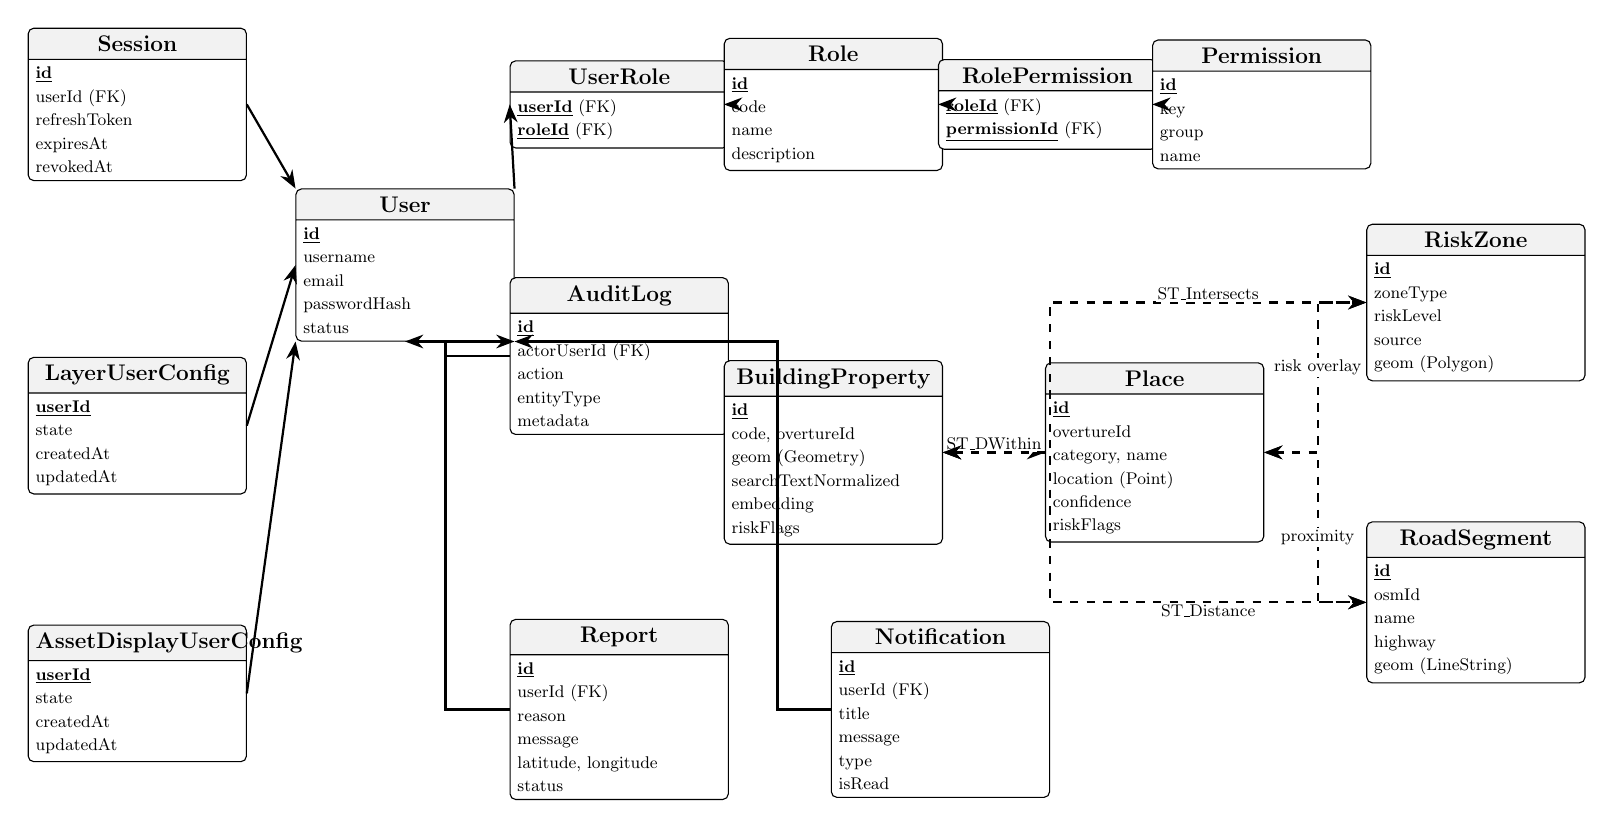
\begin{tikzpicture}[
    scale=0.68,
    transform shape,
    table/.style={
        draw,
        rectangle split,
        rectangle split parts=2,
        rectangle split part fill={gray!10, white},
        every text node part/.style={align=center, font=\bfseries},
        every two node part/.style={align=left, font=\scriptsize},
        minimum width=3.8cm,
        text width=3.8cm,
        rounded corners=2pt
    },
    rel/.style={-Stealth, thick},
    spatial/.style={Stealth-Stealth, thick, dashed},
    note/.style={font=\scriptsize, align=center, fill=white, inner sep=1pt}
]

% ================= Người dùng, phân quyền, phiên =================
\node[table] (user) at (-8, 4.5) {
    User
    \nodepart{two}
    \underline{\textbf{id}}\\
    username\\
    email\\
    passwordHash\\
    status
};

\node[table] (session) at (-13, 7.5) {
    Session
    \nodepart{two}
    \underline{\textbf{id}}\\
    userId (FK)\\
    refreshToken\\
    expiresAt\\
    revokedAt
};

\node[table] (layerconfig) at (-13, 1.5) {
    LayerUserConfig
    \nodepart{two}
    \underline{\textbf{userId}}\\
    state\\
    createdAt\\
    updatedAt
};

\node[table] (displayconfig) at (-13, -3.5) {
    AssetDisplayUserConfig
    \nodepart{two}
    \underline{\textbf{userId}}\\
    state\\
    createdAt\\
    updatedAt
};

\node[table] (userrole) at (-4, 7.5) {
    UserRole
    \nodepart{two}
    \underline{\textbf{userId}} (FK)\\
    \underline{\textbf{roleId}} (FK)
};

\node[table] (role) at (0, 7.5) {
    Role
    \nodepart{two}
    \underline{\textbf{id}}\\
    code\\
    name\\
    description
};

\node[table] (rolepermission) at (4, 7.5) {
    RolePermission
    \nodepart{two}
    \underline{\textbf{roleId}} (FK)\\
    \underline{\textbf{permissionId}} (FK)
};

\node[table] (permission) at (8, 7.5) {
    Permission
    \nodepart{two}
    \underline{\textbf{id}}\\
    key\\
    group\\
    name
};

\node[table] (audit) at (-4, 2.8) {
    AuditLog
    \nodepart{two}
    \underline{\textbf{id}}\\
    actorUserId (FK)\\
    action\\
    entityType\\
    metadata
};

% ================= Tài sản, tiện ích, phản ánh =================
\node[table] (building) at (0, 1.0) {
    BuildingProperty
    \nodepart{two}
    \underline{\textbf{id}}\\
    code, overtureId\\
    geom (Geometry)\\
    searchTextNormalized\\
    embedding\\
    riskFlags
};

\node[table] (place) at (6, 1.0) {
    Place
    \nodepart{two}
    \underline{\textbf{id}}\\
    overtureId\\
    category, name\\
    location (Point)\\
    confidence\\
    riskFlags
};

\node[table] (report) at (-4, -3.8) {
    Report
    \nodepart{two}
    \underline{\textbf{id}}\\
    userId (FK)\\
    reason\\
    message\\
    latitude, longitude\\
    status
};

\node[table] (notification) at (2, -3.8) {
    Notification
    \nodepart{two}
    \underline{\textbf{id}}\\
    userId (FK)\\
    title\\
    message\\
    type\\
    isRead
};

% ================= Không gian và rủi ro =================
\node[table] (riskzone) at (12, 3.8) {
    RiskZone
    \nodepart{two}
    \underline{\textbf{id}}\\
    zoneType\\
    riskLevel\\
    source\\
    geom (Polygon)
};

\node[table] (road) at (12, -1.8) {
    RoadSegment
    \nodepart{two}
    \underline{\textbf{id}}\\
    osmId\\
    name\\
    highway\\
    geom (LineString)
};

% ================= Quan hệ khóa ngoại =================
\draw[rel] (session.east) -- (user.north west);
\draw[rel] (layerconfig.east) -- (user.west);
\draw[rel] (displayconfig.east) -- (user.south west);
\draw[rel] (user.north east) -- (userrole.west);
\draw[rel] (userrole.east) -- (role.west);
\draw[rel] (role.east) -- (rolepermission.west);
\draw[rel] (rolepermission.east) -- (permission.west);
\draw[rel] (audit.west) -- ++(-1.2,0) |- (user.south east);
\draw[rel] (report.west) -- ++(-1.2,0) |- (user.south);
\draw[rel] (notification.west) -- ++(-1.0,0) |- (user.south east);

% ================= Quan hệ logic không gian =================
\draw[spatial] (building.east) -- (place.west) node[note, midway, above] {ST\_DWithin};
\draw[spatial] (building.east) -- ++(2.0,0) |- (riskzone.west) node[note, near end, above] {ST\_Intersects};
\draw[spatial] (building.east) -- ++(2.0,0) |- (road.west) node[note, near end, below] {ST\_Distance};
\draw[spatial] (place.east) -- ++(1.0,0) |- (riskzone.west) node[note, near start, above] {risk overlay};
\draw[spatial] (place.east) -- ++(1.0,0) |- (road.west) node[note, near start, below] {proximity};

\end{tikzpicture}%
}

\caption{Sơ đồ Thực thể Kết hợp (ERD) mô tả cấu trúc cơ sở dữ liệu hệ thống.}
    \label{fig:database_erd}
\end{figure}
\cleardoublepage
\section{DỰ TOÁN VÀ TRIỂN KHAI}

\subsection{Dự toán dự án}

\subsubsection{Căn cứ lập dự toán}
Dự án \gls{geoai} được xây dựng dựa trên các căn cứ pháp lý sau:
\begin{itemize}
    \item \gls{qd-btttt} số 671/QĐ-BTTTT ngày 26/04/2024 về hướng dẫn xác định chi phí phần mềm nội bộ.
    \item Thông tư số 36/2018/TT-BTC ngày 30/3/2018 của Bộ Tài chính về Hướng dẫn việc lập dự toán, quản lý, sử dụng và quyết toán kinh phí dành cho công tác đào tạo, bồi dưỡng cán bộ, công chức, viên chức.
    \item Thông tư số 06/2011/TT-BTTTT ngày 28/2/2011 của Bộ Thông tin và Truyền thông về việc Quy định lập và quản lý chi phí đầu tư ứng dụng \gls{cntt}.
    \item Thông tư 121/2018/TT-BTC ngày 12/12/2018 của Bộ Tài chính về Quy định về lập dự toán, quản lý, sử dụng và quyết toán kinh phí để thực hiện công tác ứng cứu sự cố, bảo đảm an toàn thông tin mạng.
    \item Công văn số 3787/BTTTT-THH ngày 26/12/2014 của Bộ Thông tin và Truyền thông về việc hướng dẫn phương pháp xác định chi phí kiểm thử chất lượng phần mềm.
    \item Công văn số 2519/BTTTT-KHTC ngày 04/9/2014 của Bộ Thông tin và Truyền thông về việc Đơn giá lắp đặt phần cứng và cài đặt phần mềm trong ứng dụng công nghệ thông tin.
    \item \gls{qd-btttt} số 1688/QĐ-BTTTT ngày 11/10/2019 về việc Sửa đổi, bổ sung Quyết định 2378/QĐ-BTTTT về định mức chi phí quản lý dự án, chi phí tư vấn đầu tư ứng dụng \gls{cntt} sử dụng ngân sách nhà nước.
    \item Quyết định số 320/QĐ-BKHCN ngày 30/3/2025 về hướng dẫn xác định đơn giá nhân công.
\end{itemize}

\subsubsection{Dự toán chi tiết}

\textbf{a. Tổng dự toán}

Bảng tổng hợp chi phí phần mềm nội bộ:
\begin{longtable}{|c|p{4.5cm}|p{3.5cm}|c|r|}
\caption{Bảng tổng hợp chi phí phần mềm nội bộ \label{tab:tong_hop_chi_phi}} \\
\hline
\textbf{TT} & \textbf{Khoản mục chi phí} & \textbf{Cách tính} & \textbf{Ký hiệu} & \textbf{Thành tiền (đồng)} \\ \hline
\endfirsthead
\hline
\textbf{TT} & \textbf{Khoản mục chi phí} & \textbf{Cách tính} & \textbf{Ký hiệu} & \textbf{Thành tiền (đồng)} \\ \hline
\endhead
\hline
\multicolumn{5}{r}{{Tiếp theo trang sau}} \\
\endfoot
\hline
\endlastfoot
1 & Chi phí trực tiếp XD, PT, MR phần mềm nội bộ & $G=1,4\times E\times P\times H$ & G & 188.976.132 \\ \hline
2 & Chi phí chung & $G\times 65\%$ & C & 122.834.486 \\ \hline
3 & Thu nhập chịu thuế tính trước & $(G+C)\times 6\%$ & TL & 18.708.637 \\ \hline
4 & Chi phí XD, PT, MR phần mềm nội bộ & $G+C+TL$ & GPM & 330.519.255 \\ \hline
5 & Chi phí dự phòng & Theo quy định & Gdp & 33.051.926 \\ \hline
\multicolumn{3}{|c|}{\textbf{TỔNG CỘNG}} & \textbf{Gpm} & \textbf{363.571.181} \\ \hline
\end{longtable}

Bảng tổng hợp dự toán:
\begin{table}[htbp]
\centering
\caption{Bảng tổng hợp dự toán \label{tab:tong_hop_du_toan}}
\vspace{0.2cm}
\resizebox{\textwidth}{!}{%
\begin{tabular}{|c|p{6cm}|c|p{5cm}|r|r|r|}
\hline
\textbf{Stt} & \textbf{Nội dung chi phí} & \textbf{Ký hiệu} & \textbf{Công thức} & \textbf{Giá trị trước thuế} & \textbf{VAT} & \textbf{Giá trị sau thuế} \\ \hline
I & Chi phí phần mềm nội bộ & GPM & Theo QĐ 671/QĐ-BTTTT & 427.730.802 & 0 & 427.730.802 \\ \hline
II & Chi phí quản lý dự án & GQL & GPM $\times$ tỷ lệ \% & 7.934.406 & 0 & 7.934.406 \\ \hline
III & Chi phí tư vấn đầu tư & GTV & \makecell{GTV1+GTV2 \\ +GTV3+GTV4} & 23.569.401 & 600.000 & 24.169.401 \\ \hline
1 & Chi phí lập báo cáo kinh tế - kỹ thuật & GTV1 & GPM $\times$ tỷ lệ \%, min 10tr & 15.569.401 & 0 & 15.569.401 \\ \hline
2 & Chi phí thẩm tra dự toán & GTV2 & GPM $\times$ tỷ lệ \%, min 2tr & 2.000.000 & 0 & 2.000.000 \\ \hline
3 & Chi phí lập hồ sơ mời thầu & GTV3 & GPM $\times$ tỷ lệ \%, min 3tr & 3.000.000 & 300.000 & 3.300.000 \\ \hline
4 & Chi phí đánh giá hồ sơ dự thầu & GTV4 & GPM $\times$ tỷ lệ \%, min 3tr & 3.000.000 & 300.000 & 3.300.000 \\ \hline
IV & Chi phí khác & GK & & 5.000.000 & 500.000 & 5.500.000 \\ \hline
1 & Chi phí kiểm thử chức năng PM & GKT & Lập dự toán & 0 & 0 & 0 \\ \hline
2 & Chi phí kiểm thử ATANTT & GKTATTT & Lập dự toán & 0 & 0 & 0 \\ \hline
3 & Chi phí thẩm định HSMT & GK1 & GPM $\times$ 0,1\%, min 2tr & 2.000.000 & 200.000 & 2.200.000 \\ \hline
4 & Chi phí thẩm định kết quả đấu thầu & GK2 & GPM $\times$ 0,1\%, min 3tr & 3.000.000 & 300.000 & 3.300.000 \\ \hline
V & Chi phí dự phòng & GDP &  \makecell{(GPM+GQL+GTV+GK) \\ $\times$ 10\%} & 46.423.461 & 0 & 46.423.461 \\ \hline
\multicolumn{2}{|c|}{\textbf{TỔNG CỘNG}} & \textbf{G} & \makecell{GPM+GQL+GTV\\ +GK+GDP} & \textbf{510.658.071} & \textbf{1.100.000} & \textbf{511.758.071} \\ \hline
\end{tabular}
}
\end{table}

\cleardoublepage
\textbf{b. Dự toán chi tiết}

\vspace{0.3cm}
\textbf{- Danh sách các tác nhân (actors):}
\begin{longtable}{|c|p{3cm}|p{6cm}|p{2cm}|c|}
\caption{Danh sách các tác nhân \label{tab:danh_sach_tac_nhan}} \\
\hline
\textbf{TT} & \textbf{Tên tác nhân} & \textbf{Mô tả tác nhân} & \textbf{Phân loại} & \textbf{Trọng số} \\ \hline
\endfirsthead
\hline
\textbf{TT} & \textbf{Tên tác nhân} & \textbf{Mô tả tác nhân} & \textbf{Phân loại} & \textbf{Trọng số} \\ \hline
\endhead
\hline
\multicolumn{5}{r}{{Tiếp theo trang sau}} \\
\endfoot
\hline
\endlastfoot
1 & Cán bộ CNTT (Admin) & Quản lý toàn bộ hệ thống, cấu hình và phân quyền & Phức tạp & 3 \\ \hline
2 & Cán bộ quản lý đô thị & Quản lý tài sản, lập kế hoạch bảo trì, xem báo cáo & Phức tạp & 3 \\ \hline
3 & Công dân & Xem bản đồ công khai, gửi phản ánh sự cố hạ tầng & Phức tạp & 3 \\ \hline
\end{longtable}

\textbf{- Danh sách yêu cầu chức năng:} Bảng ở chương III phần III mục 1. Yêu cầu chức năng của phần mềm.

\vspace{0.3cm}
\textbf{- Bảng chuyển đổi yêu cầu chức năng sang use case:} Bảng ở chương III phần II mục 2. Chuyển đổi yêu cầu chức năng sang Use Case.

\vspace{0.3cm}
\textbf{- Bảng tính điểm tác nhân không hiệu chỉnh (TAW):}
\begin{longtable}{|c|p{4cm}|c|c|c|}
\caption{Bảng tính điểm tác nhân không hiệu chỉnh (TAW) \label{tab:taw}} \\
\hline
\textbf{TT} & \textbf{Loại Actor} & \textbf{Trọng số} & \textbf{Số tác nhân} & \textbf{Điểm} \\ \hline
\endfirsthead
\hline
\textbf{TT} & \textbf{Loại Actor} & \textbf{Trọng số} & \textbf{Số tác nhân} & \textbf{Điểm} \\ \hline
\endhead
\hline
\multicolumn{5}{r}{{Tiếp theo trang sau}} \\
\endfoot
\hline
\endlastfoot
1 & Đơn giản & 1 & 0 & 0 \\ \hline
2 & Trung bình & 2 & 0 & 0 \\ \hline
3 & Phức tạp & 3 & 3 & 9 \\ \hline
\multicolumn{2}{|c|}{Cộng (1+2+3)} & & \textbf{3} & \textbf{9} \\ \hline
\multicolumn{4}{|c|}{\textbf{TAW}} & \textbf{9} \\ \hline
\end{longtable}
\cleardoublepage
\textbf{- Bảng tính điểm các trường hợp sử dụng (use case):}
\begin{longtable}{|c|p{4cm}|c|c|c|c|}
\caption{Bảng tính điểm các trường hợp sử dụng (use case) \label{tab:tbf}} \\
\hline
\textbf{STT} & \textbf{Loại} & \textbf{Trọng số} & \textbf{Hệ số BMT} & \textbf{Số UC} & \textbf{Điểm} \\ \hline
\endfirsthead
\hline
\textbf{STT} & \textbf{Loại} & \textbf{Trọng số} & \textbf{Hệ số BMT} & \textbf{Số UC} & \textbf{Điểm} \\ \hline
\endhead
\hline
\multicolumn{6}{r}{{Tiếp theo trang sau}} \\
\endfoot
\hline
\endlastfoot
1 & B - Đơn giản & 5 & 1 & 11 & 55 \\ \hline
  & B - Trung bình & 10 & 1 & 9 & 90 \\ \hline
  & B - Phức tạp & 15 & 1 & 0 & 0 \\ \hline
2 & M - Đơn giản & 5 & 1.2 & 1 & 6 \\ \hline
  & M - Trung bình & 10 & 1.2 & 0 & 0 \\ \hline
  & M - Phức tạp & 15 & 1.2 & 0 & 0 \\ \hline
3 & T - Đơn giản & 5 & 1.5 & 0 & 0 \\ \hline
  & T - Trung bình & 10 & 1.5 & 1 & 15 \\ \hline
  & T - Phức tạp & 15 & 1.5 & 0 & 0 \\ \hline
\multicolumn{2}{|c|}{Cộng (1+2+3)} & & & \textbf{22} & \textbf{166} \\ \hline
\multicolumn{5}{|c|}{\textbf{TBF}} & \textbf{166} \\ \hline
\end{longtable}
\cleardoublepage
\textbf{- Bảng hệ số phức tạp kỹ thuật – công nghệ (TCF):}
\begin{table}[htbp]
\centering
\caption{Bảng hệ số phức tạp kỹ thuật – công nghệ (TCF) \label{tab:tcf}}
\vspace{0.2cm}
\resizebox{\textwidth}{!}{%
\begin{tabular}{|c|p{5.5cm}|c|c|c|p{3.5cm}|}
\hline
\textbf{TT} & \textbf{Các hệ số KT-CN} & \textbf{Trọng số (Wi)} & \textbf{Giá trị xếp hạng (Fi)} & \textbf{Kết quả ($Wi \times Fi$)} & \textbf{Ghi chú} \\ \hline
\multicolumn{6}{|l|}{\textbf{I. Hệ số KT-CN (TFW)}} \\ \hline
T1 & Xử lý phân tán & 2 & 0 & 0 & 0-5 \\ \hline
T2 & Mức độ quan trọng của hiệu năng & 1 & 2 & 2 & 0-5 \\ \hline
T3 & Hiệu quả sử dụng cho người dùng & 1 & 2 & 2 & 0-5 \\ \hline
T4 & Độ phức tạp của xử lý bên trong & 1 & 2 & 2 & 0-5 \\ \hline
T5 & Khả năng tái sử dụng mã nguồn & 1 & 0 & 0 & 0-5 \\ \hline
T6 & Dễ cài đặt & 0.5 & 1 & 0.5 & 0-5 \\ \hline
T7 & Dễ vận hành & 0.5 & 3 & 1.5 & 0-5 \\ \hline
T8 & Khả năng chuyển đổi & 2 & 0 & 0 & 0-5 \\ \hline
T9 & Dễ dàng bảo trì & 1 & 3 & 3 & 0-5 \\ \hline
T10 & Xử lý đồng thời & 1 & 1 & 1 & 0-5 \\ \hline
T11 & Mức độ hỗ trợ bảo mật & 1 & 2 & 2 & 0-5 \\ \hline
T12 & Sự phụ thuộc vào mã lệnh bên thứ ba & 1 & 1 & 1 & 0-5 \\ \hline
T13 & Mức độ hỗ trợ đào tạo người sử dụng & 1 & 2 & 2 & 0-5 \\ \hline
\multicolumn{4}{|l|}{$TFW = \sum (Wi \times Fi)$} & \textbf{17} & \\ \hline
\multicolumn{6}{|l|}{\textbf{II. Hệ số phức tạp KT-CN (TCF)}} \\ \hline
\multicolumn{4}{|l|}{$TCF = 0.6 + (0.01 \times TFW)$} & \textbf{0.77} & \\ \hline
\multicolumn{4}{|l|}{$UUCP = TAW + TBF$} & 175 & Điểm UC chưa hiệu chỉnh \\ \hline
\multicolumn{4}{|l|}{$AUCP = UUCP \times TCF \times EF$} & \textbf{85.56625} & ĐIỂM USE CASE ĐÃ HIỆU CHỈNH \\ \hline
\end{tabular}%
}
\end{table}
\cleardoublepage

\textbf{- Bảng tính toán hệ số tác động môi trường, nhóm làm việc (ECF):}
\begin{table}[htbp]
\centering
\caption{Bảng tính toán hệ số tác động môi trường, nhóm làm việc (ECF) \label{tab:ecf}}
\vspace{0.2cm}
\resizebox{\textwidth}{!}{%
\begin{tabular}{|c|p{6cm}|c|c|c|}
\hline
\textbf{TT} & \textbf{Các hệ số môi trường} & \textbf{Trọng số (Wi)} & \textbf{Giá trị xếp hạng (Fi)} & \textbf{Kết quả ($Wi \times Fi$)} \\ \hline
E1 & Quen thuộc với quy trình phát triển PM & 1.5 & 5 & 7.5 \\ \hline
E2 & Kinh nghiệm về ứng dụng & 0.5 & 5 & 2.5 \\ \hline
E3 & Kinh nghiệm về hướng đối tượng & 1 & 3 & 3 \\ \hline
E4 & Năng lực chủ trì phân tích & 0.5 & 5 & 2.5 \\ \hline
E5 & Động lực làm việc & 1 & 5 & 5 \\ \hline
E6 & Yêu cầu ổn định & 2 & 5 & 10 \\ \hline
E7 & Nhân viên bán thời gian & -1 & 0 & 0 \\ \hline
E8 & Ngôn ngữ lập trình khó & -1 & 5 & -5 \\ \hline
\multicolumn{4}{|l|}{$EFW = \sum (Wi \times Fi)$} & \textbf{25.5} \\ \hline
\multicolumn{4}{|l|}{$ECF = 1.4 + (-0.03 \times EFW)$} & \textbf{0.635} \\ \hline
\end{tabular}%
}
\end{table}
\cleardoublepage

\textbf{- Bảng tính lương nhân công:}
\begin{table}[htbp]
\centering
\caption{Bảng tính lương nhân công \label{tab:luong_nhan_cong}}
\vspace{0.2cm}
\resizebox{\textwidth}{!}{%
\begin{tabular}{|c|p{4.5cm}|c|p{3.5cm}|r|r|r|}
\hline
\textbf{TT} & \textbf{Hạng mục} & \textbf{Ký hiệu} & \textbf{Cách tính} & \textbf{Kỹ sư bậc 1} & \textbf{Kỹ sư bậc 2} & \textbf{Kỹ sư bậc 3} \\ \hline
1 & Hệ số cấp bậc & HCB & & 2.34 & 2.65 & 2.96 \\ \hline
2 & Hệ số phụ cấp lương & HPC & & 0.00 & 0.00 & 0.00 \\ \hline
3 & Mức lương cơ sở & MLCS & & 2.340.000 & 2.340.000 & 2.340.000 \\ \hline
4 & Lương cơ bản & LCB & HCB $\times$ MLCS & 5.475.600 & 6.201.000 & 6.926.400 \\ \hline
5 & Hệ số điều chỉnh tăng thêm tiền lương & HĐC & & 0.9 & 0.9 & 0.9 \\ \hline
6 & Các khoản đóng góp theo lương & BHLĐ & BHXH + BHYT + BHTN & 1.177.254 & 1.333.215 & 1.489.176 \\ \hline
6.1 & Bảo hiểm xã hội (17,5\%) & BHXH & 17,5\% $\times$ LCB & 958.230 & 1.085.175 & 1.212.120 \\ \hline
6.2 & Bảo hiểm y tế (3\%) & BHYT & 3\% $\times$ LCB & 164.268 & 186.030 & 207.792 \\ \hline
6.3 & Bảo hiểm thất nghiệp (1\%) & BHTN & 1\% $\times$ LCB & 54.756 & 62.010 & 69.264 \\ \hline
7 & Số ngày công trong tháng & t & & 26 & 26 & 26 \\ \hline
8 & Giá ngày công & GNC & \makecell{[(HCB+HPC) $\times$ MLCS \\ $\times$ (1+HĐC) + BHLD] / t} & 445.419 & 504.428 & 563.436 \\ \hline
9 & Giá giờ công & GGC & GNC / 8 & 55.677,38 & 63.053,44 & 70.429,50 \\ \hline
10 & Số nhân công & & & 3 & 0 & 0 \\ \hline
11 & Mức lương lao động bình quân (H) & H & BQ có trọng số theo số NC & 55.677,38 & & \\ \hline
\end{tabular}%
}
\end{table}
\cleardoublepage

\textbf{- Bảng tính toán chi phí trực tiếp xây dựng phần mềm nội bộ:}
\begin{xltabular}{\textwidth}{|c|p{3.5cm}|p{3cm}|c|r|p{3cm}|}
\caption{Bảng tính toán chi phí trực tiếp xây dựng phần mềm nội bộ \label{tab:chi_phi_truc_tiep}} \\
\hline
\textbf{TT} & \textbf{Hạng mục} & \textbf{Diễn giải} & \textbf{Ký hiệu} & \textbf{Giá trị} & \textbf{Ghi chú} \\ \hline
\endfirsthead
\hline
\textbf{TT} & \textbf{Hạng mục} & \textbf{Diễn giải} & \textbf{Ký hiệu} & \textbf{Giá trị} & \textbf{Ghi chú} \\ \hline
\endhead
\hline
\multicolumn{6}{r}{{Tiếp theo trang sau}} \\
\endfoot
\hline
\endlastfoot
\multicolumn{6}{|l|}{\textbf{I. Tính điểm trường hợp sử dụng (Use case)}} \\ \hline
1 & Điểm Actor (TAW) & Phụ lục IV & TAW & 9 & \\ \hline
2 & Điểm Use case (TBF) & Phụ lục V & TBF & 166 & \\ \hline
3 & Tính điểm UUCP & $UUCP = TAW + TBF$ & UUCP & 175 & \\ \hline
4 & Hệ số phức tạp KT-CN (TCF) & $TCF = 0,6 + (0,01 \times TFW)$ & TCF & 0.77 & Phụ lục VI \\ \hline
5 & Hệ số phức tạp môi trường (EF) & $EF = 1,4 + (-0,03 \times EFW)$ & EF & 0.635 & Phụ lục VII \\ \hline
6 & Tính điểm AUCP & $UUCP \times TCF \times EF$ & AUCP & 85.56625 & \\ \hline
\textbf{II} & \textbf{Nội suy thời gian lao động (P)} & Giờ công/điểm UC & P & 20 & Nội suy từ PL VII (20-28 giờ) \\ \hline
\textbf{III} & \textbf{Giá trị nỗ lực thực tế (E)} & $E = 10/6 \times AUCP$ & E & 142.6104167 & Hệ số điều chỉnh nỗ lực \\ \hline
\textbf{IV} & \textbf{Mức lương lao động BQ (H)} & đồng/giờ & H & 55.677,38 & Theo QĐ 320/QĐ-BKHCN \\ \hline
\textbf{V} & \textbf{Chi phí trực tiếp PM nội bộ (G)} & $G = 1,4 \times E \times P \times H$ & G & 222.324.862 & đồng \\ \hline
\end{xltabular}
\cleardoublepage


\textbf{Tổng dự toán}
Bảng tổng hợp chi phí phần mềm nội bộ:
\begin{longtable}{|c|p{4.5cm}|p{3.5cm}|c|r|}
\caption{Bảng tổng hợp chi phí phần mềm nội bộ \label{tab:tong_hop_chi_phi}} \\
\hline
\textbf{TT} & \textbf{Khoản mục chi phí} & \textbf{Cách tính} & \textbf{Ký hiệu} & \textbf{Thành tiền (đồng)} \\ \hline
\endfirsthead
\hline
\textbf{TT} & \textbf{Khoản mục chi phí} & \textbf{Cách tính} & \textbf{Ký hiệu} & \textbf{Thành tiền (đồng)} \\ \hline
\endhead
\hline
\multicolumn{5}{r}{{Tiếp theo trang sau}} \\
\endfoot
\hline
\endlastfoot
1 & Chi phí trực tiếp XD, PT, MR phần mềm nội bộ & $G=1,4\times E\times P\times H$ & G & 188.976.132 \\ \hline
2 & Chi phí chung & $G\times 65\%$ & C & 122.834.486 \\ \hline
3 & Thu nhập chịu thuế tính trước & $(G+C)\times 6\%$ & TL & 18.708.637 \\ \hline
4 & Chi phí XD, PT, MR phần mềm nội bộ & $G+C+TL$ & GPM & 330.519.255 \\ \hline
5 & Chi phí dự phòng & Theo quy định & Gdp & 33.051.926 \\ \hline
\multicolumn{3}{|c|}{\textbf{TỔNG CỘNG}} & \textbf{Gpm} & \textbf{363.571.181} \\ \hline
\end{longtable}

Bảng tổng hợp dự toán:
\begin{table}[htbp]
\centering
\caption{Bảng tổng hợp dự toán \label{tab:tong_hop_du_toan}}
\vspace{0.2cm}
\resizebox{\textwidth}{!}{%
\begin{tabular}{|c|p{6cm}|c|p{5cm}|r|r|r|}
\hline
\textbf{Stt} & \textbf{Nội dung chi phí} & \textbf{Ký hiệu} & \textbf{Công thức} & \textbf{Giá trị trước thuế} & \textbf{VAT} & \textbf{Giá trị sau thuế} \\ \hline
I & Chi phí phần mềm nội bộ & GPM & Theo QĐ 671/QĐ-BTTTT & 427.730.802 & 0 & 427.730.802 \\ \hline
II & Chi phí quản lý dự án & GQL & GPM $\times$ tỷ lệ \% & 7.934.406 & 0 & 7.934.406 \\ \hline
III & Chi phí tư vấn đầu tư & GTV & \makecell{GTV1+GTV2 \\ +GTV3+GTV4} & 23.569.401 & 600.000 & 24.169.401 \\ \hline
1 & Chi phí lập báo cáo kinh tế - kỹ thuật & GTV1 & GPM $\times$ tỷ lệ \%, min 10tr & 15.569.401 & 0 & 15.569.401 \\ \hline
2 & Chi phí thẩm tra dự toán & GTV2 & GPM $\times$ tỷ lệ \%, min 2tr & 2.000.000 & 0 & 2.000.000 \\ \hline
3 & Chi phí lập hồ sơ mời thầu & GTV3 & GPM $\times$ tỷ lệ \%, min 3tr & 3.000.000 & 300.000 & 3.300.000 \\ \hline
4 & Chi phí đánh giá hồ sơ dự thầu & GTV4 & GPM $\times$ tỷ lệ \%, min 3tr & 3.000.000 & 300.000 & 3.300.000 \\ \hline
IV & Chi phí khác & GK & & 5.000.000 & 500.000 & 5.500.000 \\ \hline
1 & Chi phí kiểm thử chức năng PM & GKT & Lập dự toán & 0 & 0 & 0 \\ \hline
2 & Chi phí kiểm thử ATANTT & GKTATTT & Lập dự toán & 0 & 0 & 0 \\ \hline
3 & Chi phí thẩm định HSMT & GK1 & GPM $\times$ 0,1\%, min 2tr & 2.000.000 & 200.000 & 2.200.000 \\ \hline
4 & Chi phí thẩm định kết quả đấu thầu & GK2 & GPM $\times$ 0,1\%, min 3tr & 3.000.000 & 300.000 & 3.300.000 \\ \hline
V & Chi phí dự phòng & GDP &  \makecell{(GPM+GQL+GTV+GK) \\ $\times$ 10\%} & 46.423.461 & 0 & 46.423.461 \\ \hline
\multicolumn{2}{|c|}{\textbf{TỔNG CỘNG}} & \textbf{G} & \makecell{GPM+GQL+GTV\\ +GK+GDP} & \textbf{510.658.071} & \textbf{1.100.000} & \textbf{511.758.071} \\ \hline
\end{tabular}
}
\end{table}

\cleardoublepage
\subsection{Tiến độ triển khai}
\begin{longtable}{|c|p{6cm}|c|c|}
\caption{Tiến độ triển khai \label{tab:tien_do}} \\
\hline
\textbf{Stt} & \textbf{Hạng mục công việc} & \textbf{Thời gian bắt đầu} & \textbf{Thời gian kết thúc} \\ \hline
\endfirsthead
\hline
\textbf{Stt} & \textbf{Hạng mục công việc} & \textbf{Thời gian bắt đầu} & \textbf{Thời gian kết thúc} \\ \hline
\endhead
\hline
\multicolumn{4}{r}{{Tiếp theo trang sau}} \\
\endfoot
\hline
\endlastfoot
1 & Khảo sát yêu cầu, lập hồ sơ thuyết minh thiết kế kỹ thuật, tổng dự toán & 02/2025 & 03/2025 \\ \hline
2 & Phân tích và thiết kế hệ thống & 03/2025 & 03/2025 \\ \hline
3 & Thiết kế giao diện & 03/2025 & 03/2025 \\ \hline
4 & Xây dựng phần mềm & 03/2025 & 06/2025 \\ \hline
5 & Nghiệm thu và đưa phần mềm vào sử dụng & 06/2025 & 06/2025 \\ \hline
\end{longtable}

\subsection{Phương án tổ chức thực hiện}

\subsubsection{Phương án cài đặt, triển khai}
\begin{itemize}
    \item Triển khai trên hạ tầng đám mây lai (hybrid cloud): máy chủ on-premise của TTDL \gls{tptp} cho dữ liệu nhạy cảm, kết hợp cloud công cộng cho khả năng mở rộng.
    \item CI/CD pipeline tự động hóa quá trình build, test và deploy.
    \item Blue-Green Deployment để đảm bảo zero-downtime khi cập nhật phiên bản.
\end{itemize}

\subsubsection{Phương án đào tạo}
Đào tạo cho 3 nhóm đối tượng:
\begin{itemize}
    \item Nhóm 1 - Quản trị viên hệ thống (10 người): Khóa đào tạo 3 ngày tập trung về quản trị hệ thống, cấu hình \gls{gis} server, quản lý dữ liệu không gian, xử lý sự cố. Tài liệu: Hướng dẫn quản trị hệ thống (150 trang).
    \item Nhóm 2 - Cán bộ quản lý đô thị (50 người): Khóa đào tạo 2 ngày về sử dụng \gls{webgis}, tra cứu và quản lý tài sản, xem báo cáo và dashboard. Tài liệu: Hướng dẫn sử dụng (100 trang).
    \item Nhóm 3 - Cán bộ khảo sát thực địa (100 người): Đào tạo 1 ngày về sử dụng mobile app, quy trình thu thập dữ liệu tại thực địa. Tài liệu: Hướng dẫn nhanh (30 trang) + video tutorial.
\end{itemize}
\cleardoublepage
\subsubsection{Phương án vận hành, quản lý, khai thác}
\begin{itemize}
    \item Bố trí 2 cán bộ chuyên trách vận hành hệ thống \gls{geoai} tại Trung tâm \gls{cntt}-TT \gls{tptp}.
    \item Hệ thống giám sát tự động (Prometheus + Grafana) cảnh báo 24/7 về hiệu năng, lỗi và bảo mật.
    \item Họp đánh giá hàng tháng giữa đơn vị vận hành và các sở ngành sử dụng để cải tiến liên tục.
    \item Cập nhật model \gls{ai} định kỳ 6 tháng/lần dựa trên dữ liệu mới thu thập.
\end{itemize}

\subsubsection{Phương án kiểm thử các yêu cầu chức năng và phi chức năng}
\begin{itemize}
    \item Kiểm thử chức năng: Sử dụng công cụ Selenium/Playwright cho automation test \gls{webgis}; Postman cho \gls{api} test; QGIS cho kiểm tra dữ liệu không gian.
    \item Kiểm thử hiệu năng: Apache JMeter mô phỏng 500 người dùng đồng thời, đặc biệt kiểm thử render bản đồ với 100.000+ điểm dữ liệu.
    \item Kiểm thử bảo mật: OWASP ZAP cho quét tự động; chuyên gia bảo mật độc lập thực hiện penetration testing.
    \item Kiểm thử \gls{ai}: Đánh giá độ chính xác model (accuracy, precision, recall, F1-score) trên tập dữ liệu kiểm thử 1.000 ảnh được gán nhãn.
\end{itemize}

\subsubsection{Cam kết bảo hành và hỗ trợ kỹ thuật}
\begin{itemize}
    \item Bảo hành 24 tháng kể từ ngày nghiệm thu, bao gồm sửa lỗi phần mềm, hỗ trợ kỹ thuật và cập nhật bản vá bảo mật.
    \item SLA hỗ trợ: phản hồi trong 2 giờ cho lỗi nghiêm trọng, 8 giờ cho lỗi trung bình, 24 giờ cho yêu cầu thông thường.
    \item Cập nhật model \gls{ai} miễn phí trong 24 tháng bảo hành khi dữ liệu training mới đạt đủ ngưỡng.
    \item Hotline kỹ thuật 24/7 trong suốt thời gian bảo hành.
    \item Sau thời gian bảo hành, đơn vị phát triển cam kết cung cấp dịch vụ bảo trì, nâng cấp theo hợp đồng hỗ trợ riêng.
\end{itemize}
\cleardoublepage
\section*{PHỤ LỤC I - SƠ ĐỒ USE CASE HỆ THỐNG GEOAI}
\addcontentsline{toc}{section}{PHỤ LỤC I - SƠ ĐỒ USE CASE HỆ THỐNG GEOAI}

\subsubsection*{1. Use Case Quản lý tài sản đô thị trên bản đồ}
\begin{itemize}
    \item Tác nhân: Cán bộ quản lý đô thị, Cán bộ khảo sát thực địa, Quản trị viên.
    \item Use case chính: Xem bản đồ, Thêm tài sản mới, Cập nhật tài sản, Tra cứu tài sản, Xuất dữ liệu.
    \item Extend: Upload ảnh tài sản, Phân tích \gls{ai} tự động, Gắn thẻ QR code.
\end{itemize}

\subsubsection*{2. Use Case Module AI và Cảnh báo tự động}
\begin{itemize}
    \item Tác nhân: Hệ thống \gls{ai} tự động, Camera/\gls{iot}, Cán bộ quản lý.
    \item Use case chính: Phân tích ảnh tài sản, Phát hiện sự cố, Gửi cảnh báo, Dự báo bảo trì.
    \item Include: Lưu kết quả phân tích \gls{ai}, Cập nhật tình trạng tài sản, Tạo phiếu công việc.
\end{itemize}

\subsubsection*{3. Use Case Cổng Công dân}
\begin{itemize}
    \item Tác nhân: Công dân/người dân, Cán bộ tiếp nhận phản ánh.
    \item Use case chính: Xem bản đồ công khai, Gửi phản ánh sự cố, Tra cứu tiến độ xử lý.
    \item Extend: Xác thực địa chỉ GPS, Đính kèm ảnh sự cố, Nhận thông báo cập nhật.
\end{itemize}
\cleardoublepage
\section*{PHỤ LỤC II - BẢNG THỐNG KÊ DỮ LIỆU TÀI SẢN ĐÔ THỊ}
\addcontentsline{toc}{section}{PHỤ LỤC II - BẢNG THỐNG KÊ DỮ LIỆU TÀI SẢN ĐÔ THỊ}
Ước tính quy mô dữ liệu tài sản đô thị cần quản lý tại \gls{tptp} (giai đoạn đầu):
\begin{longtable}{|c|p{4cm}|p{3.5cm}|p{5cm}|}
\caption{Bảng thống kê dữ liệu tài sản đô thị \label{tab:phu_luc_2}} \\
\hline
\textbf{STT} & \textbf{Loại tài sản đô thị} & \textbf{Số lượng ước tính} & \textbf{Ghi chú} \\ \hline
\endfirsthead
\hline
\textbf{STT} & \textbf{Loại tài sản đô thị} & \textbf{Số lượng ước tính} & \textbf{Ghi chú} \\ \hline
\endhead
\hline
\multicolumn{4}{r}{{Tiếp theo trang sau}} \\
\endfoot
\hline
\endlastfoot
1 & Cây xanh đô thị & $\sim$450.000 cây & Toàn \gls{tptp} \\ \hline
2 & Đèn chiếu sáng công cộng & $\sim$120.000 bóng & Đường phố và công viên \\ \hline
3 & Biển báo giao thông & $\sim$80.000 biển & Các loại biển báo, hiệu lệnh \\ \hline
4 & Hố ga thoát nước & $\sim$200.000 hố ga & Hệ thống thoát nước \\ \hline
5 & Trụ điện công cộng & $\sim$60.000 trụ & Lưới điện hạ thế \\ \hline
6 & Bảng điện tử quảng cáo & $\sim$5.000 bảng & Màn hình LCD, bảng led \\ \hline
7 & Đường giao thông (phân đoạn) & $\sim$15.000 đoạn & Theo lý trình đường \\ \hline
8 & Cầu, hầm chui & $\sim$1.200 công trình & Cầu các loại \\ \hline
9 & Trạm bơm, cống điều tiết & $\sim$3.000 công trình & Hệ thống thủy lợi nội thị \\ \hline
10 & Camera giám sát công cộng & $\sim$18.000 camera & Đường phố và giao lộ \\ \hline
\end{longtable}
\cleardoublepage
\section*{PHỤ LỤC III - YÊU CẦU HẠ TẦNG TRIỂN KHAI}
\addcontentsline{toc}{section}{PHỤ LỤC III - YÊU CẦU HẠ TẦNG TRIỂN KHAI}
\begin{longtable}{|c|p{4cm}|p{4cm}|p{4.5cm}|}
\caption{Yêu cầu hạ tầng triển khai \label{tab:phu_luc_3}} \\
\hline
\textbf{STT} & \textbf{Thành phần} & \textbf{Cấu hình tối thiểu} & \textbf{Ghi chú} \\ \hline
\endfirsthead
\hline
\textbf{STT} & \textbf{Thành phần} & \textbf{Cấu hình tối thiểu} & \textbf{Ghi chú} \\ \hline
\endhead
\hline
\multicolumn{4}{r}{{Tiếp theo trang sau}} \\
\endfoot
\hline
\endlastfoot
1 & GeoServer (GIS Engine) & 8 CPU, 32GB RAM, SSD 500GB & Có thể cluster 2 node \\ \hline
2 & \gls{ai} Processing Server & GPU NVIDIA A 100/ 16 CPU/64GB RAM & Cho inference \gls{ai} real-time \\ \hline
3 & PostgreSQL + PostGIS & 16 CPU, 64GB RAM, NVMe 2TB & CSDL không gian địa lý \\ \hline
4 & Application Server (API) & 8 CPU, 32GB RAM x 2 (HA) & FastAPI + load balancer \\ \hline
5 & MinIO Object Storage & 4 CPU, 16GB RAM, HDD 10TB & Lưu ảnh tài sản \\ \hline
6 & Redis Cache & 4 CPU, 16GB RAM & Cache bản đồ và phiên \\ \hline
7 & Kafka Message Queue & 8 CPU, 32GB RAM, SSD 500GB & Stream \gls{iot} data \\ \hline
8 & Monitoring Stack & 4 CPU, 8GB RAM & Prometheus + Grafana \\ \hline
\end{longtable}

\vspace{1cm}
\begin{flushright}
- \centering Hết - \\
\centering Đà Nẵng, tháng 6 năm 2025
\end{flushright}
\clearpage

% phantomsection giúp hyperlink bấm vào đúng vị trí hơn
% \phantomsection 
% \addcontentsline{toc}{section}{TÀI LIỆU THAM KHẢO}
% \nocite{*} 
% \bibliographystyle{ieeetr}
% \bibliography{references/TLTK}

\end{document}